\documentclass[a4paper,10pt]{book}
\usepackage[utf8]{inputenc}
\usepackage{fullpage}
\usepackage{cite}
\usepackage[utf8]{inputenc}
\usepackage{a4wide}
\usepackage{url}
\usepackage{graphicx}
\usepackage{caption}
\usepackage{float} % para que los gr\'aficos se queden en su lugar con [H]
\usepackage{subcaption}
\usepackage{wrapfig}
\usepackage{color}
\usepackage{amsmath} %para escribir funci\'on partida , matrices
\usepackage{amsthm} %para numerar definciones y teoremas
\usepackage[hidelinks]{hyperref} % para inlcuir links dentro del texto
\usepackage{tabu} 
\usepackage{comment}
\usepackage{amsfonts} % \mathbb{N} -> conjunto de los n\'umeros naturales  
\usepackage{enumerate}
\usepackage{listings}
\usepackage[colorinlistoftodos, textsize=small]{todonotes} % Para poner notas en el medio del texto!! No olvidar hacer. 
\usepackage{framed} % Para encuadrar texto. \begin{framed}
\usepackage{csquotes} % Para citar texto \begin{displayquote}
\usepackage{epigraph} % Epigrafe  \epigraph{texto}{\textit{autor}}
\usepackage{authblk}
\usepackage{titlesec}
\usepackage{varioref}
\usepackage{bm} % \bm{\alpha} bold greek symbol
\usepackage{pdfpages} % \includepdf
\usepackage[makeroom]{cancel} % \cancel{} \bcancel{} etc
\usepackage{wrapfig} % \begin{wrapfigure} Pone figura al lado del texto
\usepackage{mdframed}
\usepackage{algorithm}
%\usepackage{quoting}
\usepackage{mathtools}	
\usepackage{tikz}
\usepackage{paracol}

\newcommand{\vm}[1]{\mathbf{#1}}
\newcommand{\N}{\mathcal{N}}
\newcommand{\citel}[1]{\cite{#1}\label{#1}}
\newcommand\hfrac[2]{\genfrac{}{}{0pt}{}{#1}{#2}} %\frac{}{} sin la linea del medio

\newtheorem{midef}{Definition}
\newtheorem{miteo}{Theorem}
\newtheorem{mipropo}{Proposition}

\theoremstyle{definition}
\newtheorem{definition}{Definition}[section]
\newtheorem{theorem}{Theorem}[section]
\newtheorem{proposition}{Proposition}[section]


%http://latexcolor.com/
\definecolor{azul}{rgb}{0.36, 0.54, 0.66}
\definecolor{rojo}{rgb}{0.7, 0.2, 0.116}
\definecolor{rojopiso}{rgb}{0.8, 0.25, 0.17}
\definecolor{verdeingles}{rgb}{0.12, 0.5, 0.17}
\definecolor{ubuntu}{rgb}{0.44, 0.16, 0.39}
\definecolor{debian}{rgb}{0.84, 0.04, 0.33}
\definecolor{dkgreen}{rgb}{0,0.6,0}
\definecolor{gray}{rgb}{0.5,0.5,0.5}
\definecolor{mauve}{rgb}{0.58,0,0.82}

\lstset{
  language=Python,
  aboveskip=3mm,
  belowskip=3mm,
  showstringspaces=true,
  columns=flexible,
  basicstyle={\small\ttfamily},
  numbers=none,
  numberstyle=\tiny\color{gray},
  keywordstyle=\color{blue},
  commentstyle=\color{dkgreen},
  stringstyle=\color{mauve},
  breaklines=true,
  breakatwhitespace=true,
  tabsize=4
}

% tikzlibrary.code.tex
%
% Copyright 2010-2011 by Laura Dietz
% Copyright 2012 by Jaakko Luttinen
%
% This file may be distributed and/or modified
%
% 1. under the LaTeX Project Public License and/or
% 2. under the GNU General Public License.
%
% See the files LICENSE_LPPL and LICENSE_GPL for more details.

% Load other libraries

%\newcommand{\vast}{\bBigg@{2.5}}
% newcommand{\Vast}{\bBigg@{14.5}}
% \usepackage{helvet}
% \renewcommand{\familydefault}{\sfdefault}

\usetikzlibrary{shapes}
\usetikzlibrary{fit}
\usetikzlibrary{chains}
\usetikzlibrary{arrows}

% Latent node
\tikzstyle{latent} = [circle,fill=white,draw=black,inner sep=1pt,
minimum size=20pt, font=\fontsize{10}{10}\selectfont, node distance=1]
% Observed node
\tikzstyle{obs} = [latent,fill=gray!25]
% Invisible node
\tikzstyle{invisible} = [latent,minimum size=0pt,color=white, opacity=0, node distance=0]
% Constant node
\tikzstyle{const} = [rectangle, inner sep=0pt, node distance=0.1]
%state
\tikzstyle{estado} = [latent,minimum size=8pt,node distance=0.4]
%action
\tikzstyle{accion} =[latent,circle,minimum size=5pt,fill=black,node distance=0.4]
\tikzstyle{fijo} =[latent,circle,minimum size=5pt,fill=black]


% Factor node
\tikzstyle{factor} = [rectangle, fill=black,minimum size=10pt, draw=black, inner
sep=0pt, node distance=1]
% Deterministic node
\tikzstyle{det} = [latent, rectangle]

% Plate node
\tikzstyle{plate} = [draw, rectangle, rounded corners, fit=#1]
% Invisible wrapper node
\tikzstyle{wrap} = [inner sep=0pt, fit=#1]
% Gate
\tikzstyle{gate} = [draw, rectangle, dashed, fit=#1]

% Caption node
\tikzstyle{caption} = [font=\footnotesize, node distance=0] %
\tikzstyle{plate caption} = [caption, node distance=0, inner sep=0pt,
below left=5pt and 0pt of #1.south east] %
\tikzstyle{factor caption} = [caption] %
\tikzstyle{every label} += [caption] %

\tikzset{>={triangle 45}}

%\pgfdeclarelayer{b}
%\pgfdeclarelayer{f}
%\pgfsetlayers{b,main,f}

% \factoredge [options] {inputs} {factors} {outputs}
\newcommand{\factoredge}[4][]{ %
  % Connect all nodes #2 to all nodes #4 via all factors #3.
  \foreach \f in {#3} { %
    \foreach \x in {#2} { %
      \path (\x) edge[-,#1] (\f) ; %
      %\draw[-,#1] (\x) edge[-] (\f) ; %
    } ;
    \foreach \y in {#4} { %
      \path (\f) edge[->,#1] (\y) ; %
      %\draw[->,#1] (\f) -- (\y) ; %
    } ;
  } ;
}

% \edge [options] {inputs} {outputs}
\newcommand{\edge}[3][]{ %
  % Connect all nodes #2 to all nodes #3.
  \foreach \x in {#2} { %
    \foreach \y in {#3} { %
      \path (\x) edge [->,#1] (\y) ;%
      %\draw[->,#1] (\x) -- (\y) ;%
    } ;
  } ;
}

% \factor [options] {name} {caption} {inputs} {outputs}
\newcommand{\factor}[5][]{ %
  % Draw the factor node. Use alias to allow empty names.
  \node[factor, label={[name=#2-caption]#3}, name=#2, #1,
  alias=#2-alias] {} ; %
  % Connect all inputs to outputs via this factor
  \factoredge {#4} {#2-alias} {#5} ; %
}

% \plate [options] {name} {fitlist} {caption}
\newcommand{\plate}[4][]{ %
  \node[wrap=#3] (#2-wrap) {}; %
  \node[plate caption=#2-wrap] (#2-caption) {#4}; %
  \node[plate=(#2-wrap)(#2-caption), #1] (#2) {}; %
}

% \gate [options] {name} {fitlist} {inputs}
\newcommand{\gate}[4][]{ %
  \node[gate=#3, name=#2, #1, alias=#2-alias] {}; %
  \foreach \x in {#4} { %
    \draw [-*,thick] (\x) -- (#2-alias); %
  } ;%
}

% \vgate {name} {fitlist-left} {caption-left} {fitlist-right}
% {caption-right} {inputs}
\newcommand{\vgate}[6]{ %
  % Wrap the left and right parts
  \node[wrap=#2] (#1-left) {}; %
  \node[wrap=#4] (#1-right) {}; %
  % Draw the gate
  \node[gate=(#1-left)(#1-right)] (#1) {}; %
  % Add captions
  \node[caption, below left=of #1.north ] (#1-left-caption)
  {#3}; %
  \node[caption, below right=of #1.north ] (#1-right-caption)
  {#5}; %
  % Draw middle separation
  \draw [-, dashed] (#1.north) -- (#1.south); %
  % Draw inputs
  \foreach \x in {#6} { %
    \draw [-*,thick] (\x) -- (#1); %
  } ;%
}

% \hgate {name} {fitlist-top} {caption-top} {fitlist-bottom}
% {caption-bottom} {inputs}
\newcommand{\hgate}[6]{ %
  % Wrap the left and right parts
  \node[wrap=#2] (#1-top) {}; %
  \node[wrap=#4] (#1-bottom) {}; %
  % Draw the gate
  \node[gate=(#1-top)(#1-bottom)] (#1) {}; %
  % Add captions
  \node[caption, above right=of #1.west ] (#1-top-caption)
  {#3}; %
  \node[caption, below right=of #1.west ] (#1-bottom-caption)
  {#5}; %
  % Draw middle separation
  \draw [-, dashed] (#1.west) -- (#1.east); %
  % Draw inputs
  \foreach \x in {#6} { %
    \draw [-*,thick] (\x) -- (#1); %
  } ;%
}


\usepackage{physics}
\newcommand*\diff{\mathop{}\!\mathrm{d}}

\newif\ifen
\newif\ifes
\newcommand{\en}[1]{\ifen#1\fi}
\newcommand{\es}[1]{\ifes#1\fi}
\estrue


%opening
\title{\huge Inferencia.}
\author{Gustavo Landfried}

\begin{document}

\maketitle

\tableofcontents

\chapter{Conocimiento empírico}


\section{Introducción}

La ciencia es una institución humana que tiene pretensión de verdad, esto es de formular proposiciones que tengan validez universal.
%
La validación del conocimiento formal se realiza a través de la demostración de teoremas en sistemas axiomáticos cerrados.
%
La validación del conocimiento empírico tiene la dificultad de que debe realizarse en sistemas abiertos, por lo que siempre existe un grado de incertidumbre asociada.
%
La honestidad, entendida como maximización de la incertidumbre (entropía) dadas las evidencia empíricas (datos) y las evidencias formales (modelos causales) es la fuente de validez del conocimiento empírico.

\section{Conocimiento empírico}

En algún momento hace aproximadamente 4500 millones de años, apareció en la tierra una forma de organización de la materia capaz de auto-replicarse.
%
El crecimiento de un linaje es un proceso multiplicativo y ruidoso, una secuencia de probabilidades de supervivencia y reproducción.
%
Los errores producidos durante la replicación diversifican las formas de organización de la materia, y las diferentes tazas de superviencia favorecen a aquellas formas que están mejor adaptas al medio.
%
En este sentido, la vida puede ser vista como un sistema distribuido de procesamiento de información, y las diversas formas que adquiere la vida puede ser visto como una forma de conocimiento empírico.

% Parrafo

Hasta hace poco se consideró una verdad establecida que la cooperación requería algún tipo de comportamiento altruista para evolucionar.
%
Esta conclusión suponía implícitamente que los sistemas evolutivos son ergódicos.
%
La teoría ergódica es una rama muy técnica de las matemáticas.
%
Por suerte, para el propósito de esta discusión, necesitamos sólo conocer su definición.
%
Diremos que un proceso es ergódico si su media temporal es igual al valor esperado,
%
\begin{equation}
 \lim_{T \mapsto \infty} \int_0^T f(\omega(t)) \diff t  = \int_{\Omega} f(\omega)p(\omega) \diff\omega
\end{equation}
%
donde $\omega \in \Omega$ representa los estados del sistema, $\omega(t)$ el estado del sistema obtenido aleatoriamente en el tiempo $t$, $p(\cdot)$ la distribución de probabilidad de los estados, y $f(\cdot)$ una transformación a los estados.

% Parrafo

Reconocer si el sistema es ergódico o no es importante porque en los procesos no-ergódicos lo que le ocurre a los agentes en el tiempo no coincide con la esperanza de los estados del sistema~\cite{peters2019-ergodicityEconomics}.
%
Por ejemplo, en la teoría evolutiva se enseña a todos el hecho de que el crecimiento de un linaje es un proceso multiplicativo y ruidoso, una secuencia de probabilidades de supervivencia y reproducción.
%
El proceso multiplicativo de la vida no es ergódicos porque los impactos de las pérdidas son a menudo más fuertes que los de las ganancias: con que haya un cero en la secuencia de supervivencia y reproducción, cualquier linaje está extinto para siempre.
%
Los procesos evolutivos, por lo tanto, ofrecen una ventaja física concreta a favor del comportamiento cooperativo: dado que la varianza realmente importa para la supervivencia, una forma eficaz de reducirla es cooperar compartiendo los riesgos~\cite{yaari2010-cooperationEvolution,peters2015-evolutionaryAdvantageOfCooperation}.

% Parrafo

Por ejemplo, consideremos el siguiente ejemplo de jugete.
%
La naturaleza lanza una moneda: si sale cara tu riqueza crece un 50\%, si sale cruz tu riqueza pierde un 40\%.
%
\begin{equation}
\Delta x =
\begin{cases}
 +0.5x & \text{ \en{Head}\es{Cara} } \\
 -0.4x & \text{ \en{Tail}\es{Seca} }
\end{cases}
\end{equation}
%
El valor esperado, utilizado todavía por las corrientes principales tanto de la teoría económica como de la teoría de toma de decisiones, predicen que los agentes van a tener un cambio positivo de alrededor de $\langle \Delta x \rangle = 0.05x$.
%
Sin embargo, lo que le ocurre a los agentes individuales en el tiempo es muy diferente a lo esperado: a largo plazo todos pierden.
%
En la figura \ref{fig:simple_gamble} mostramos las trayectorias individuales en el tiempo.
%
\begin{figure}[ht!]
    \centering
    \begin{subfigure}[b]{0.48\textwidth}
    \includegraphics[width=\linewidth]{figures/simple_gamble.pdf}
    \caption{Trayectorias individuales}
    \label{fig:simple_gamble}
    \end{subfigure}
    \begin{subfigure}[b]{0.48\textwidth}
    \includegraphics[width=\linewidth]{figures/simple_gamble_incesto.pdf}
    \caption{Trayectorias cooperativas}
    \label{fig:simple_gamble_incesto}
    \end{subfigure}
    \caption{
    Riqueza de los agentes en el tiempo: en la figura \ref{fig:simple_gamble} los agentes juegan individualmente, en la figura \ref{fig:simple_gamble_incesto} los agentes comparten un porcentaje de su riqueza en cada paso.
    }
    \label{fig:gamble}
\end{figure}
%
En la figura \ref{fig:simple_gamble_incesto} mostramos las trayectorias individuales cuando los agentes comparten parte de su riqueza con el resto.
%
Por el contrario, cuando los agentes comparten parte de su riqueza con otros, todos se benefician.
%
Para entender por qué ocurre esto veamos en detalle un ejemplo.
%
En la tabla \ref{tab:gamble} podemos ver cómo se modifica la riqueza individual de dos agentes en el tiempo cuando no cooperan y cuando cooperan.
%
\begin{table}[ht!] \centering
    \begin{tabular}{|l|c|c|c|c|c|c|c|}
     \hline
        {\small Agentes} & {\small \en{Wealth}\es{Riqueza}} & {\small \en{Growth}\es{Aumento}} & {\small \en{Wealth}\es{Riqueza}} & {\small \en{Sharing}\es{Reparto}} & {\small \en{Growth}\es{Aumento}} & {\small \en{Wealth}\es{Riqueza}} & {\small \en{Sharing}\es{Reparto}} \\ \hline \hline
        A no-coop& $1$ & $\Delta +0.5$ & $1.5$ & $1.5$ & $\Delta -0.4$ & $0.9$ & $\bm{0.9}$ \\ \hline
        B no-coop & $1$ & $\Delta -0.4$ & $0.6$ & $0.6$ & $\Delta +0.5$ & $0.9$ & $\bm{0.9}$ \\ \hline\hline
        A coop & $1$ & $\Delta +0.5$ & $1.5$ & $1.05$ & $\Delta -0.4$ & $0.63$ & $\bm{1.1}$ \\ \hline
        B coop & $1$ & $\Delta -0.4$ & $0.6$ & $1.05$ & $\Delta +0.5$ & $1.58$ & $\bm{1.1}$\\ \hline
    \end{tabular}
    \caption{
    Evolución de la riqueza en procesos multiplicativos para agentes que no cooperan (primera dos filas) y agentes que sí cooperan (segundas dos filas).
    }
    \label{tab:gamble}
\end{table}
%
Ambas personas comienzan con la misma riqueza y modifican su riqueza del mismo modo pero en distito orden: en la primer paso la riqueza del agentes A aumenta y la del agente B se reduce, y viceversa.
%
Los agentes que no dividen su riqueza en la columna ``Reparto'' terminan perdiendo 10\% de su riqueza inicial, mientras que los agentes que sí dividen su riqueza finalizan con 10\% más de su riqueza inicial.
%
Mediante la cooperación los agentes tienen acceso a otros estados del sistema, lo que hace que sus trayectorias temporales $\overline{x}$ se aproximen ahora sí al valor esperado $\langle x \rangle$.

% Parrafo

En los procesos multiplicativos, como el de selección natural o el visto en el ejemplo anterior, hay una ventaja física a favor de los comportamientos cooperativos.
%
La complejidad actual de la vida~\cite{barOn2018-biomasa} es consecuencia de una serie de transiciones evolutivas~\cite{maynardSmith1995-majorTransitions} en las que entidades que antes eran capaces de replicarse de forma independiente,luego de la transición sólo pueden replicarse como partes de una unidad mayor.
%
\es{La tabla~\ref{tab:transitions} enumera algunas de las principales transiciones ocurridas en la historia evolutiva de la vida.}
%
\begin{table}[ht!] \centering
    \begin{tabular}{l}
        \hline
        \en{From molecules to populations of molecules} 
        \es{De moléculas a poblaciones de moléculas}
        \\%        
        \en{From prokaryotes to eukaryotes}
        \es{De procariotas a eucariotas}
        \\%
        \en{From asexual clones to sexual populations}
        \es{De clones asexuales a poblaciones sexuales}
        \\%
        \en{From unicellular to multicellular entities}
        \es{De entidades unicelulares a multicelulares}
        \\%
        \en{From individual to societies}
        \es{De individuos a sociedades}
        \\
        \hline
    \end{tabular}
    \caption{
    \es{Algunas de la principales transiciones evolutivas}
    }
    \label{tab:transitions}
\end{table}
%
Junto a estas saltos en los niveles de complejidad se observan cambios en el almacenamiento y transmisión de información y la aparición de formas de ``división social del trabajo'' al interior de las poblaciones.

%

Lo que hace que los humanos sean especialmente inteligentes no es sólo las capacidades cognitivas individuales, sino fundamentalmente la información cultural heredada.
%
Cada uno de nuestros antepasados imit\'o, modific\'o y transmiti\'o parte de su conocimiento a la siguiente generaci\'on, llegando a nosotros sedimentado en forma de herramientas, creencias y rutinas esenciales para la vida.
%
Otros animales también son capaces de crear herramientas, transmitir conocimiento entre generaciones y desarrollar tradiciones culturales.
%
Sin embargo, el nivel de complejidad y diversificación de la acumulación cultura humana no tiene comparación.
%
Nuestra extraordinaria capacidad para imitar, combinada con los largos per\'iodos de aprendizaje juvenil y vida posreproductiva, permite a los humanos aprender de los dem\'as y transmitir las innovaci\'on a trav\'es de la generaciones~\cite{Richerson2020}.

% Parrafo

\todo[inline]{La selección de los modelos científicos sigue la misma estrucutra que la selección de las especies.}


% Parrafo

La información cultural fue la que le permitió a los humanos adaptarse a todos los nichos ecológicos de la tierra sin necesidad de modificar su sistema de información genético.
%
Este éxito, basado en el sistema de información cultural, se ve relativizado cuando consideramos que nuestra especie representa sólo el 0.01\% de la biomasa actual de la tierra.
%
En la figura~\ref{fig:biomass} vemos estimaciones recientes~\ref{barOn2018} de la distribución de la biomasa en el planeta tierra.
%
\begin{figure}[ht!]
    \centering
    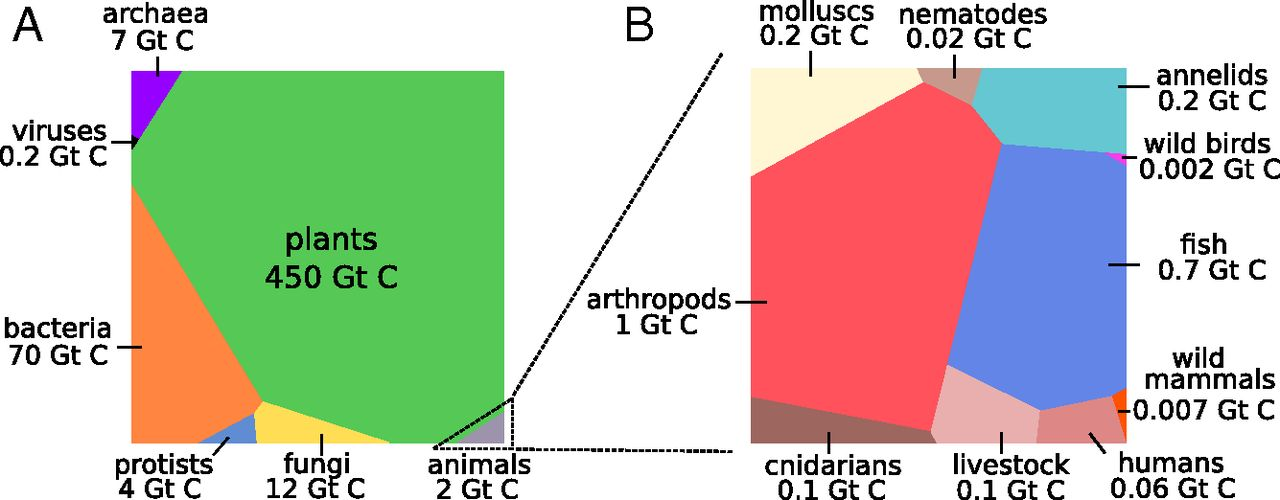
\includegraphics[width=0.7\linewidth]{static/biomass}
    \caption{
    \es{Distribución de la biomasa en el planeta tierra.}
    }
    \label{fig:biomass}
\end{figure}
%
En el gráfico de la izquierda podemos ver que la plantas y las bacterias representan el 95\% de la biomasa de la tierra.
%
En este sentido, el conocimiento que estas especies almacenan en su sistema genético es varios órdenes de magnitud superior al alcanzado por los seres humanos mediante el sistema de información cultural.
%
A pesar de que el tamaño de la población humana aumentó enormemente durante los últimos siglos, nuestra especie representamos apenas el 3\% de toda la biomasa animal.


\section{Cultura}

\en{Empathy is the cognitive skill that allowed the development of Homo sapiens: mutual understanding, imitation, language and finally culture.}%
\es{La empatía es la habilidad cognitiva que permitió el desarrollo del Homo sapiens: la comprensión mutua, la imitación, el lenguaje y finalmente la cultura.}%
%
\en{}%
\es{Nada de esto hubiera sido posible sin una actitud activa de mututo entendimiento~\cite{tomasello2005-sharingIntentions}.}%

% Parrafo

\en{}%
\es{La especial integraci\'on de los procesos biol\'ogicos, cognitivos y sociales que permiten a los humanos desarrollar culturas complejas no hubiera sido posible sin el desarrollo previo de la crianza cooperativa~\cite{hrdy2020-emotionallyModern}.}%
%
\en{}%
\es{La forma en la que estos homininos organizaron la crianza produjo un ambiente que favoreció la selección de los jóvenes capaces de monitorear las intenciones de los demás para atraer la atención de sus cuidadores.}%
%
\en{}%
\es{Antes del surgimiento de los humanos \emph{anatómicamente} modernos (masa cerebral actual) y de los humanos \emph{conductualmente} modernos (lenguaje), surgió en África una linaje \emph{emocionalmente} moderno~\cite{}, que comenzó a interesarse por los pensamientos e intenciones de los demás, y ansiosos por compartir sus propios sentimientos.}%
%
\en{}%
\es{Los ejemplos de animales que, como los humanos, ofrecen voluntariamente sus alimentos preferidos a otros se observa casi exclusivamente en especies que tienen historias evolutivas de crianza cooperativa (asistencia y provisionamiento cooperativo de las crías).}%

%

\es{La crianza cooperativa permitió del desarrollo del entendimiento mutuo, base para el comportamiento cooperativo.}%
%
\es{El desarrollo de la empatía, del entendimiento mutuo y luego del lenguaje permitió que los agentes compartieran el conocimiento entre personas pero también de generación en generación.}%
%
\es{Lo que antes debía ser redescubierto una y otra vez mediante costosa experiencia individual, ahora podría ser transmitido a la siguiente generación mediante las capacidades especiales de aprendizaje social.}%
%
\es{A partir de ese momento el conocimiento deja de ser una propiedad individual y pasa a ser una propiedad poblacional.}%
%
\es{Las sociedades humanas comienzan a funcionar desde entonces como \emph{sistemas naturales de procesamiento de informaci\'on distribuida}, acumulando información cultural que supera ampliamente a lo que cualquier persona individualmente podría descubrir en un período de vida.}%
%
\es{Lo que nos hace especialmente ``inteligentes'' a nuestra especie no es tanto las capacidades cognitivas sino la informaci\'on cultural heredada.}%

%

\es{El surgimiento de la cultura produjo cambios radicales para nuestra especie.}%
%
\es{El genoma de los chimpancés es hoy más diverso que el de los humanos justamente porque nuestra especie estuvo en grave peligro de extinción antes de esta transición cultural.}%
%
\es{Luego de la transición cultural, organizados en sociedades cazadoras recolectoras, nuestra especie salió de África y en pocos años ocupó todos los nichos ecológicos de la tierra.}%
%
\es{La información transgeneracional fue lo que le permitió a estas sociedades adaptarse rápidamente a los desafíos ecológicos.}%
%
\es{En el inicio del Holoceno, hace unos 11000 años, comienza a desarrollarse la agricultura en los 6 grandes sistemas geográficos.}%
%
\begin{figure}[ht!]
    \centering
    \includegraphics[width=0.7\linewidth]{figures/agricultura.pdf}
    \caption{Surgimiento de la agricultura.}
    \label{fig:agricultura}
\end{figure}
%
\es{Alrededor de ellos se desarrollan los principales centros poblacionales de la humanidad.}%
%
\es{A su vez, el aumento de la población promovió el desarrollo de nuevas innovaciones tecnológicas, como la escritura, la matem\'aticas, las ingenier\'ias, la astronomía, las ciencias políticas, entre otras.}%
%
\es{Algunas comunidades periféricas comienzan a integrarse a los centros de innovación, produciendo interdependencias culturales.}%
%
\es{El asilamiento, total o parcial, de una de estas poblaciones puede generar en ellas una perdida masiva de información cultural.}%
%
\es{Un ejemplo de aislamiento total bien documentado ocurre con la separación de Tanzania del continente Australiano por la subida del nivel del mar producida a comienzas del Holonceno \cite{henrich}.}%
%
\es{Un caso de asilamiento parcial ocurre cuando el mundo Árabe y el Imperio Romano de Oriente desconectan la región occidental del Imperio Romano (actuales Italia, Alemania, Francia, Inglaterra) del sistema euro-asiático.}%
%
\es{Esa etapa coincide con el proceso de involución cultural conocido como ``Edad media''}%

% 

\es{Durante el año 1400 el mundo florecía de sociedades "prósperas"~\cite{dussel2004-sistemaMundo}.}%
% los Aztecas en MesoAmerica, Los Incas en SudAmerica, el imperio de Tonga en el pacífico, los Bantú en África, los Árabes e Indios en eurasia Occidental y Chinos en Eurasia Oriental, solo por mencionar algunos.
%
\es{El imperio Incaico ocupaba gran parte de Sud América basados en tecnologías de organización orginal que no requerían una moneda: el intercambio dentro de las comunidades y entre ellas se realizaba exclusivamente mediante la ayuda mutua y la reciprocidad del trabajo, minka y ayni; e incluso los "impuestos" del Estado eran pagados por las comunidades mediante el trabajo directo, mita.}%
%
\es{El imerio Azteca ocupaba Meso América basados en extensos sistemas comerciales, grandes mecados, y ciudades llegaron a alcanzar 300.000 habitantes, tres veces la ciudad de Venecia en esa misma época.}%
% http://www7.uc.cl/sw_educ/historia/conquista/parte1/html/h54.html
%"Tiene otra plaza tan grande como dos veces la ciudad de Salamanca, toda cercada de portales alrededor, donde hay cotidianamente arriba de 60.000 Hernán Cortés, Cartas de relación de la conquista de México, Ed.Espasa-Calpe, Madrid, 1942, págs.100-101.
%
\es{El imperio de Tonga ocupaba hace siglos todo el oc\'eano pac\'ifico.}%
\es{Los pueblos Bantúes ocupaban en África toda la región subsahariana.}%
%
\es{El mundo \'Arabe comerciaba productos de una punta a la otra del globo, desde el Oc\'eano Atl\'antico, en Marruecos, hasta el Océano Pacífico en las Filipinas, conectando las innovaciones culturales, cient\'ificas y t\'ecnicas de diferentes regiones del mundo euro-asiático.}%

%

\es{Quizás el centro más avanzado en términos científicos y tecnologías haya sido la región de China~\cite{needham2004-generalConclusionsAndReflections}.}%
%
\es{China fue desde por lo menos el siglo segundo antes de cristo el centro del mundo productivo del mundo, de donde los Romanos se abastec\'ian de seda.}%
%
\es{Desarrolla el acero en el siglo segundo, el papel en el siglo sexto, la imprenta en el siglo octavo, el papel moneda en el noveno, la br\'ujula en el onceavo.}%
%
\es{Para el año 1400, China llevaba al menos 2000 de continuidad socio-pol\'itica, y 900 a\~nos de un estado meritocr\'atico, en el cual sus miembros eran elegidos a trav\'es de un examen imperial.}%
%
\es{China era una región autónoma y autosuficiente, impulsora de innovaciones.}%
%
\es{Es así como China si bien desarrolla una de las flotas más increibles de la Historia durante el 1400, luego de la serie de expediciones de Zheng He (1405-1433) el Gobierno Chino decide cerrarse fronteras adentro y dándolas por finalizadas definitivamente.}%
%
\es{No parecían necesitar nada afuera de sus fronteras.}%
\begin{figure}[ht!]     
  \centering 
  \begin{subfigure}[b]{0.35\textwidth}
    \includegraphics[width=\textwidth]{static/zhengHe_columbus.png} 
    \caption{}
    \label{fig:zhengHe_columbus}
  \end{subfigure}
  \begin{subfigure}[b]{0.5\textwidth}
    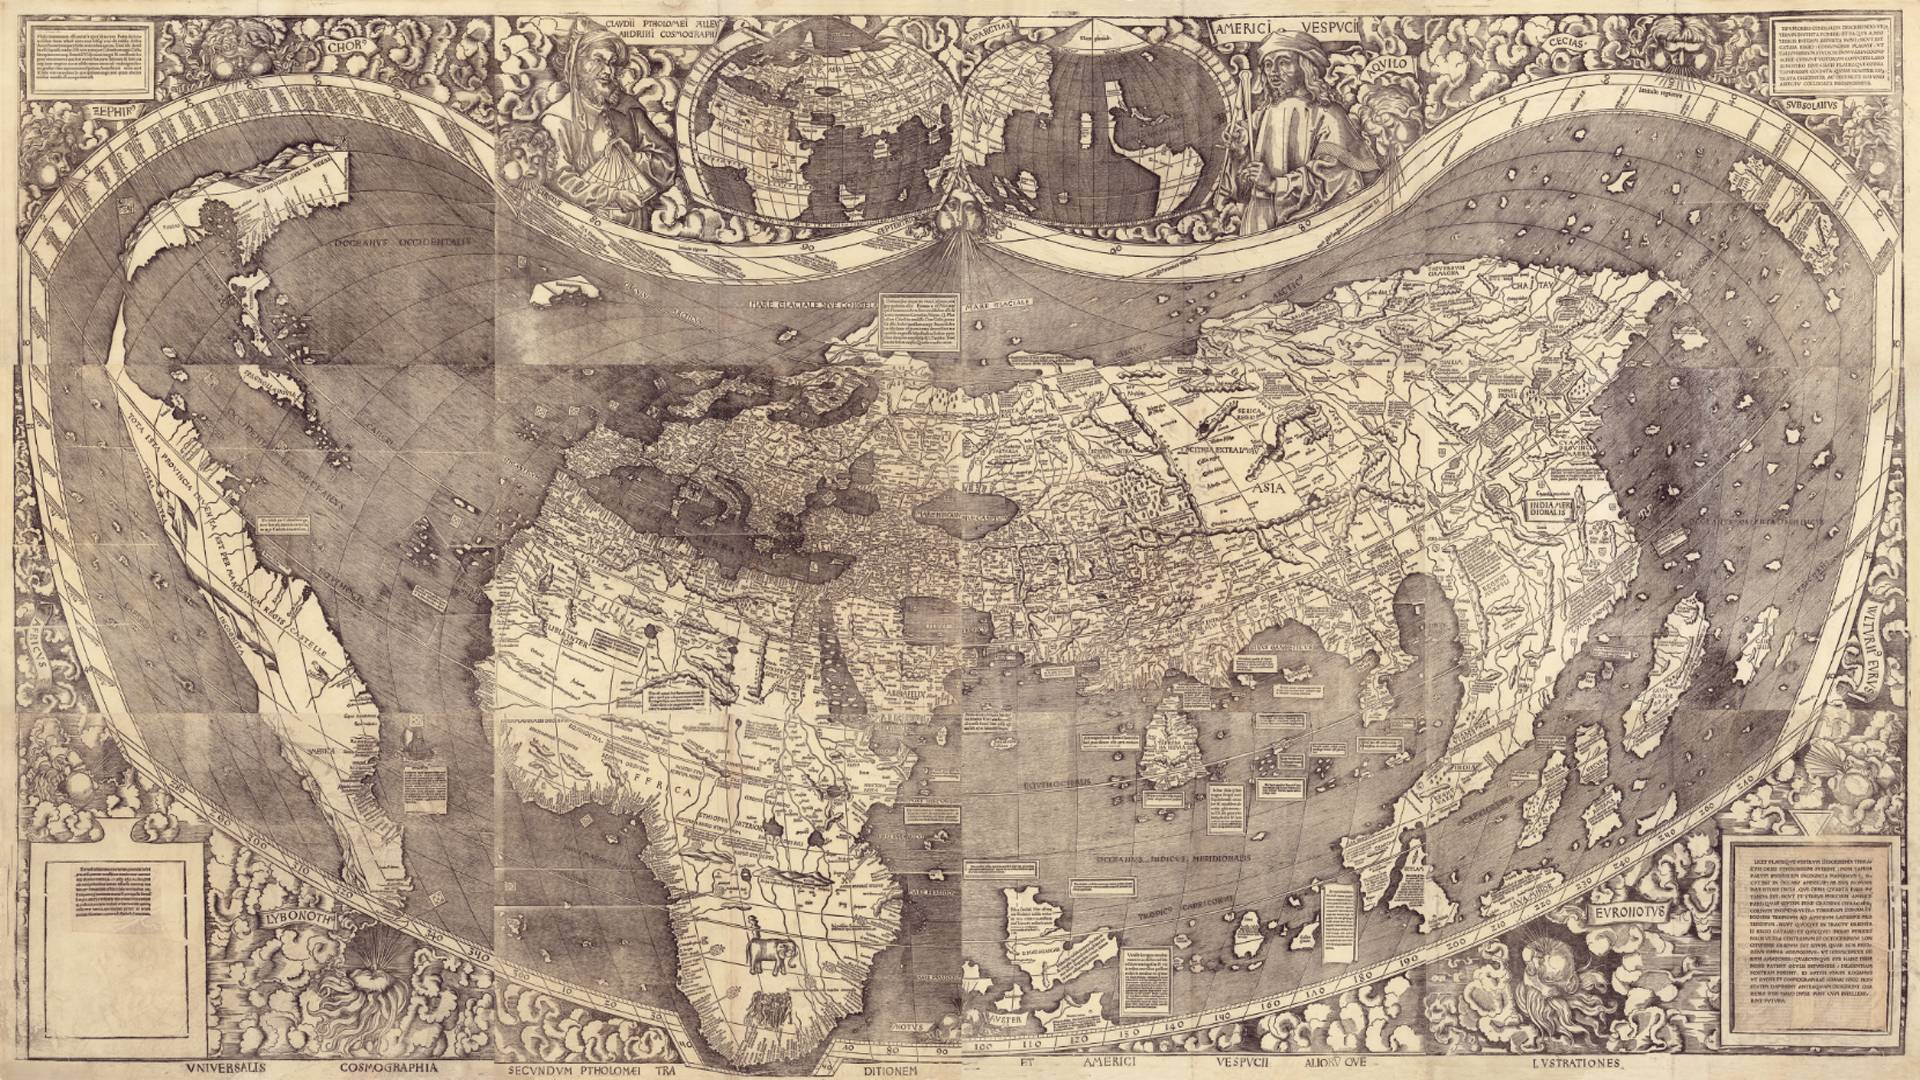
\includegraphics[width=\textwidth]{static/mapaWaldseemuller.jpg} 
    \caption{}
    \label{fig:mapaWaldseemuller}
  \end{subfigure}
  \caption{
  En la figura \ref{fig:zhengHe_columbus} se puede ver el tama\~no relativo de los barcos de la flota China del a\~no 1400 comparado con los utilizados por Cristóbal Col\'on \cite{pomeranz2000-divergence}.
  En la figura \ref{fig:mapaWaldseemuller} mostramos el primer mapa conocido de América, que fue dibujado en Europa continentalen en 1507~\cite{waldseemuller1959-universalisCosmographia}, varios años antes de que el primer europeo viera costa pacífica (el contorno de sud américa se aprecia mejor en el globo terraqueo arriba al centro).
  }
  \label{zhengHe_columbus}
\end{figure}

% Parrafo

\es{En la etapa en la que Europa occidental quedó aislada del sistema mundo se produjo al interior un proceso conocido como ``edad media'' de perdida masivas de información cultural y de degradación de las condiciones socio-económicas de la población.}%
%En el siglo XV anterior a 1492, lo que llamamos Europa occidental, la península latino-germánica, era un mundo periférico y dependiente del mundo islámico.
%Europa occidental, un territorio pequeño con algo más de setenta millones de habitantes (la mitad de lo que China tenía en ese momento), era una cultura paulatinamente aislada desde el siglo VII por la expansión árabe.
%Su débil conexión con el ``sistema mundo'' ocurría a través del Mediterráneo oriental, mediada por los puestos de Venecia, Génova, Amalfi y otros.
%Por el contrario, los comerciantes musulmanes conectaban el Océanos Atlántico y Pacífico, desde España y Marruecos hasta las Filipinas.
%El centro poblacional y comercial más denso del sistema, sin embargo, se encontraba en China y en Indostán.
%La Europa latino-germánica era una cultura secundaria, arrinconada en el lejano Occidente.
\es{Exactamente al contrario de lo que ocurrió con China, apenas Europa occidental descubre cómo navegar el Atlántico, comienza un proceso migratorio masivo producto de la pésima situación socio-económica de la ``edad media''.}%
%
\es{Los exploradores feudales quedaron asombrados por la espontánea generosidad de los habitantes Americanos.}%
%
% \es{La sorpresa de tuvo Colón es similar a la que luego reportarán otro marineros: ``Cuando les pides algo que tienen, nunca dicen que no. Al contrario, se ofrecen a compartir con cualquiera''.}%
% %
% \es{Pero Colón, producto de la sociedad feudal tenía intenciones muy diferentes: ``No llevan armas, ni las conocen (...). Serían buenos siervos (...). Con cincuenta hombres podríamos subyugarlos a todos y hacerles hacer lo que quisiéramos''.}%
%
\es{Además de la buena predisposición con la que fueron recibidos, la llegada masiva de migrantes feudales produjo en América una serie de pandemias que redujeron la población en más de 60\% entre los años 1500 y el 1600~\cite{koch2019-europeanArrival}.}%
%
\es{Esta catástrofe sanitaria generó pérdida de información cultural en América y debilitamiento de las comunidades locales, favoreciendo el avance de los exploradores feudales.}%

% Parrafo

\es{Un siglo antes, China hab\'ia incorporado la plata como monedad oficial, que era utilizada como moneda de cambio en todo el mundo Árabe~\cite{pomeranz2000-divergence, pomeranz2018-tradeCreated}.}%
%
\es{Por otra parte, en Sud América el imperio Inca ocupaba una región montañosa rica en minerales preciosos que usaba marginalmente debido a que la organización del estado se realizaba mediante el intercambio recíproco en ausencia de moneda~\cite{murra1978-organizacion}.}%
%
\es{La plata de Potosí, descubierta en 1546, colocó inmediatamente a la Europa feudal en una posición privilegiado en todo el mundo afro-euro-asiático.}%
%
%De repente la sociedad de la edad media pasa del aislamiento absoluto, de transitar una trayectoria temporal a solas, a ser la sociedad con una capacidad de intercambio extraordinaria, a transitar una trayectoria temporal con acceso privilegiado a los estados del sistema.
%
\begin{figure}[ht!]     
  \centering 
  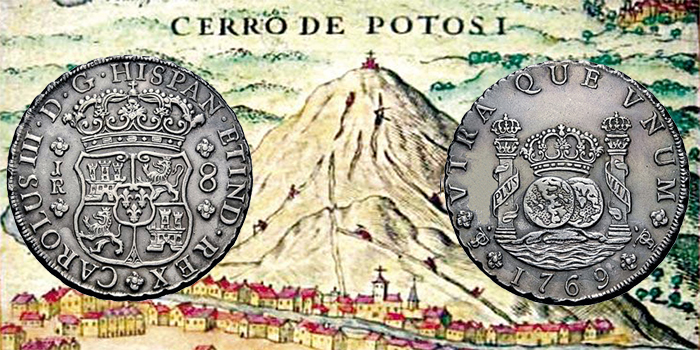
\includegraphics[width=0.5\textwidth]{static/plata-potosi} 
  \caption{
  La plata de Potosí, descubierta en 1546, pone de reprente en una posición privilegiada a la Europa feudal en todo el mundo afro-euro-asiático.
  }
  \label{fig:china-pop}
\end{figure}
%
\es{No sólo le permite romper el asilamiento sufrido durante la edad media (la batalla de Lepanto ocurre en 1571), la integración al sistema mundo inicia un proceso rápido de acumulación cultural basado en las tecnologías extranjeras.}%
%
\es{La plata de América fluye en todas las direcciones, principalmente en dirección a China.}%
%
\es{No hay ning\'un instrumento de la revoluci\'on agr\'icola inglesa, considerada causa de la revolución industrial, que no tenga origen Chino.}%
%
\es{Durante 250 años esa plata sirvió para muchas cosas, pero principalmente para comprar productos chinos y financiar la primera industrialización británica con tecnología china.}%

%

\es{Durante siglos, Europa había consumido especias, seda y otros productos asiáticos, pero exportaba muy poco a Asia.}%
%
\es{El comercio internacional de opio comenzó en el 1700 como respuesta a una crisis del comercio internacional europeo (especialmente británico).}%
%
\es{El opio, un producto lujoso utilizado en China como medicina (raramente como estupefaciente), fue prohibida por los emperadores chinos en 1729 debido a su abundancia, que hacía crecer lentamente la cantidad de adictos.}%
%
\es{Las consecuencias fueron más graves cuando en 1818 alguien desarrolló una mezcla de opio más barata y potente.}%
%
\begin{figure}[ht!]     
  \centering 
  \includegraphics[width=0.6\textwidth]{figures/china.pdf} 
  \caption{
  }
  \label{fig:china-pop}
\end{figure}
%
%\es{Los resultados fueron tan espectaculares como los que más tarde conseguiría el cártel de la droga de Medellín al convertir la costosa cocaína en crack barato.}%
%
\es{Ahora salía suficiente plata de China para compensar el déficit comercial que Gran Bretaña tenía con China.}%
%
\es{El número de adictos llegó a ser lo suficientemente alarmante, y en 1839 China comete el error de declarar la guerra al narco-estado británico, con resultados terribles.}%
%
% The Taiping Rebellion (1851–​1864) may be the most destructive civil war ever, claiming more than 20 million lives
\es{Los chinos no sólo no pudieron impedir el ingreso de la droga,  perdieron también su autonomía arancelaria, el derecho a someter a los residentes extranjeros a la ley china.}%
%
\es{Expuesta a su debilidad militar, China sufrió un siglo calamitoso de agresiones extranjeras, desorden interno y guerra civil, que produjo una caída de 1/5 de su población.}%

%

\es{Con las guerras del opio, en 1839, se establece finalmente la hegemonía de Europa occidenta.}%
%
\es{A partir de entonces comienza un avance sin precedentes de Europa sobre los pueblos de todo el mundo.}%
%
\es{Es una nueva era de avances científicos y tecnológicos, pero por otro es la era de los genocidios y de la pérdida de la diversidad cultural.}%
%
\es{Comienza la colonización de África continental en 1850.}%
%
\es{En América Latina se producen los mayores genocidios y ocupación de territorios, que todavía seguían a manos de comunidades locales.}%
%
\begin{figure}[ht!]
    \centering
    \begin{subfigure}[b]{0.48\textwidth}
    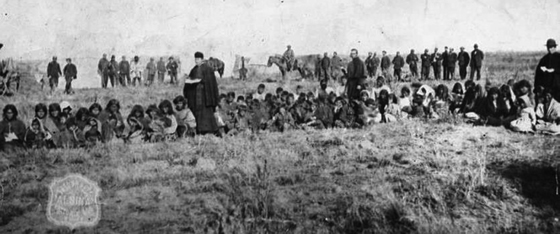
\includegraphics[width=\linewidth]{static/genocidio_patagonia}
    \caption{Genoetnocidios}
    \label{fig:genocidio_patagonia}
    \end{subfigure}
    \begin{subfigure}[b]{0.47\textwidth}
    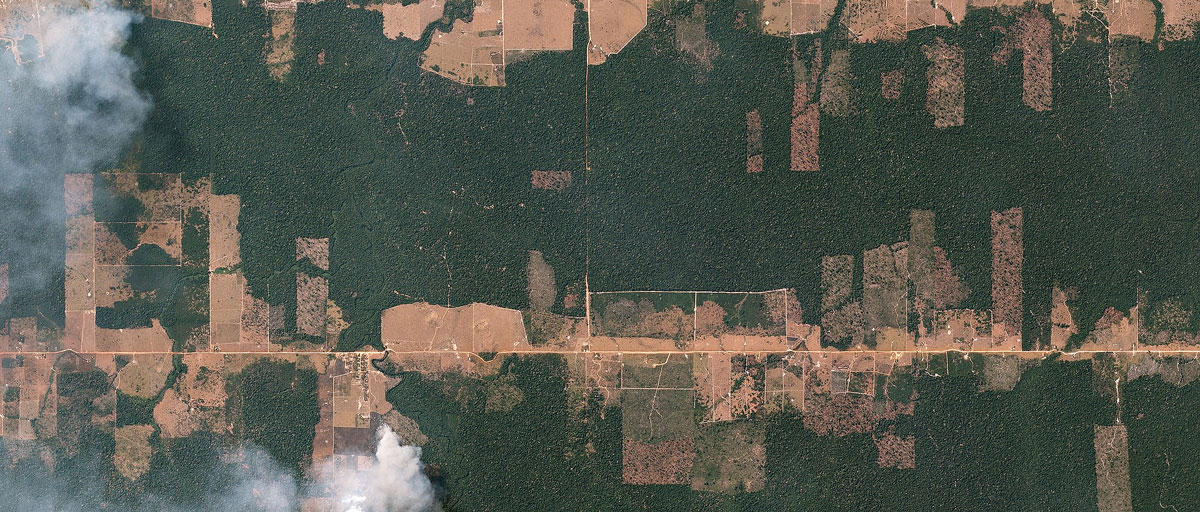
\includegraphics[width=\linewidth]{static/deforestation-brazil}
    \caption{Crisis ecológica}
    \label{fig:deforestation-brazil}
    \end{subfigure}
    \caption{
    }
    \label{fig:cultural-lose}
\end{figure}
\es{En todas las partes del globo, los etnógrafos fueron documentando la perdida de cultural debida al avance del frente colonial-moderno, estatal o privado, sobre las autonomías locales.}%

% Parrafo

\es{La pérdida de biodiversidad actual está precedida por la pérdida de diversidad cultural.}%
%
\es{A pesar de todos los avances científicos, la masiva pérdida de conocimiento cultural trajo como consecuencia una crisis ecológica sin precedentes.}%
%
La ciencia metropolitana moderna no fue capaz de compensar la perdida de las conocimientos milenarios desarrollados por las comunidades autónomas locales.
%
\es{La re-adaptación ecológica requiere recuperar las autonomías comunitarias perdidas en el proceso colonial-moderno~\cite{segato2013}.}%
%
\es{A través de pluralismo histórico\cite{segato2013}, de una gobernanza policéntrica\cite{ostrom}, se podrá recuperar el proceso de evolución cultural, fuente de la inteligencia de nuestra especie.}%
%\es{En la actualidad la situación es la inversa, debido a las transformaciones de la naturaleza, son los chimancé quienes corren un peligro de extinción.}%

\section{No mentir}

% \es{Entre los primates superiores, los humanos se destacan por su disposición constante a intercambiar pequeños favores y hacer regalos.}%
% %
% \es{Estas acciones que re-actualizan los vínculos y lazos reciprocitarios son tecnologías de sociabilidad surgidas de la politicidad doméstica~\cite{segato2016-guerraContraLasMujeres}.}%
% %
% \es{Uno de los principales temas de la literatura etnográfica estudia los diversos sistemas de intercambio de las diferentes culturas del mundo.}%
% %
% \es{Los pueblos desarrollan vastas y complejas terminologías para identificar a los parientes y a sus colaboradores, lo que les permite ampliar las relaciones basadas en la confianza, que pueden activarse y mantenerse en funcionamiento mediante el intercambio recíproco o dejarse inactivas hasta que se las necesiten.}%
% 
% % Parrafo
% 
% ERGODICIDAD ARRIBA
% 
% % Parrafo
% 
% \es{Algo similar ocurre con el proceso evolutivo de la información cultural.}%
% %


Una de las normas presentes en todas las sociedades humanas es el principio de ``no mentir''.
%
La experiencia acumulada a través de las generaciones por las más diversas comunidades del mundo condujo, de forma independiente, a la aparición de tecnologías de sociabilidad sorprendentemente similares, funamentales para el cumplimiento de este tipo de ``normas sociales''.
%
En todas ellas se pueden reconocer al menos dos mecanismos que cumplen la función de re-ciclar los v\'inculos interprersonales: los ritos festivos y los ritos coercitivos \cite{segato}.
%
Los ritos coercitivos requieren de la autonomía jurisdicción comunitaria para orientar el restablecimiento de los vínculos mediante los mecanismos de ``reparación'', ``conciliación'' y ``ayuda'' \cite{zaffaroni2013}.
%
Estos no son más que nombres para los tres tipos de intercambios posibles entre partes: ($\rightarrow$) el acto en el cual el acusado (o sus representantes) da algo al acusante (o sus representantes); ($\leftrightarrow$) el acto en el cual el acusado y acusante (o sus representantes) dan y reciben mutuamente; ($\leftarrow$) el acto en el cual el acusado (o sus representantes) recibe algo del acusante (o sus representantes).
%
Los ritos coercitivos no son otra cosa que ceremonias de intercambio.
%
La estrategia de estos sistemas consiste en re-activar el flujo de intercambios entre las partes, rotos previamente por un conflicto.
%
La expulsión del agresor de la comunidad sólo se prevee en casos extremadamente excepcionales, pues el primer derecho de sus miembros es el derecho a la comunidad \cite{segato}.

%

\subsection{El criterio de autoridad colonial-estatal y la crisis ecológica}

En este sentido, la sociedad feudal fue una anomalía reciente en la historia de la humanidad.
%
En esta etapa comenzó a ganar terreno al interior de esta sociedad el criterio de autoridad (sexual, militar, académica, moral) como fundamento del ``saber auténtico''.
%
El incumplimiento de las normas dejó de estar regulado por los ritos coercitivos y pasó a estar monopolizado por el poder militar-religioso, que impuso el monopolio absoluto sobre los cuerpos, excluyendo a la víctima y a la comunidad de la decisión y la administración del restablecimiento de los vínculos.

%

\es{Durante esa etapa, las instituciones heredades del Imperio Romano de Occidente comenzaron a competir con las comunidades indígenas locales y la Iglesia Católica produce una serie de importantes tecnologías de colonización~\cite{zaffaroni2013-cuestionCriminal}.}%
%
\begin{figure}[ht!]
    \centering
    \includegraphics[width=0.2\linewidth]{static/digesto.jpg}
    
\includegraphics[width=0.21\linewidth]{static/malleus.jpeg}
    \caption{La guerra contra las mujeres como tecnología de colonización. %La proscripción de las tecnología de sociabilidad comunitaria, acción política del espacio doméstico administrada principalmente por las mujeres, debilita el arraigo comunitario facilitando la capatación de población desertora para actividades militares.
    }
    \label{fig:malleus}
\end{figure}
%
\es{La primera acción importante es la intervención en las relaciones comunitaria de reproducción, regulando las relaciones familiares y sexuales.}%
%
\es{Al proscribir la acción política del espacio doméstico,  núcleo fundamental de toda tecnología de sociabilidad comunitaria administrada principalmente por las mujeres, se debilita el arraigo comunitario, facilitando la captación de población desertora para actividades militares.}%
%
\es{El poder punitivo se fue extendiendo y un nuevo sistema penal re-nació de los llamados \emph{libris terribilis} del Digesto, antiguas leyes romanas recolectadas por encargo del emperador Justiniano de Constantinopla y re-interpretadas de modo de liberar el poder punitivo de todo límite.}%
%
\es{La guerra contra las mujeres se formaliza definitivamente con la publicación del \emph{Malleus maleficarum} en 1484, que fue el segundo best seller más impreso después de la Biblia durante los siguientes 200 años.}%
%
\es{El sujeto masculino se torna modelo de lo humano y de todo cuanto sea dotado de politicidad, interés general y valor universal, y el espacio de las mujeres se transforma en margen y resto de la política.}%

%

Sólo después de que la sociedad feudal sale de su aislamiento, gracias a las epidemias que produce su migración en América y luego al acceso de la plata americana que los pone en una posición de privilegiada en todo el mundo Afro-Euro-Asiático, comienza al interior de esta sociedad un debate sobre las fuentes de validación del conocimiento.
%
\en{}%
\es{En esta etapa el criterio de experiencia personal comenzó ganar terreno como fundamento del ``saber auténtico'' sobre los criterios de autoridad.}%
%
Sin embargo el avance fue sólo parcial.
%
\es{Este criterio que fue utilizado para democratizar el conocimiento al interior de la sociedad feudal en el nuevo contexto, sin embargo se reservan para uso exclusivo de sus miembros varones.}
%
\es{El argumento de la superioridad moral sigue siendo usando como justificación de dominación colonial-patriarcal, y se continua en la actualidad como imposición de la jurisdicción estatal sobre las comunidades locales.}
%
El argumento lo desarrolla por primera vez Ginés de Sepúlveda, cuatro años después del descubrimiento de la plata de Potosí, en 1550.%
%
\begin{quotation}
 Será siempre justo y conforme al derecho natural que tales gentes [bárbaras] se sometan al imperio de príncipes y naciones más cultas y humanas, para que por sus virtudes y la prudencia de sus leyes, depongan la barbarie y se reduzcan a vida más humana y al culto de la virtud [...] Y si rechazan tal imperio se les puede imponer por medio de las armas, y tal guerra será justa según el derecho natural lo declara [...] En suma: es justo, conveniente y conforme a la ley natural que los varones probos, inteligentes, virtuosos y humanos dominen sobre todos los que no tienen estas cualidades\cite{GinesdeSepulveda1967p87}.
\end{quotation}
%
\es{Este argumento se impondrá a pesar de que avanzado el proceso colonial-moderno, a partir de Kant, se llegue al consenso de que la fuente de validez del conocimiento se fundamenta en la norma conocida como el imperativo categórico,}%
%
\begin{quotation}
Obra de tal modo que la máxima de tu voluntad pueda valer siempre al mismo tiempo como principio de una legislación universal. \cite{Kant2003:28}
\end{quotation}
%
La ``universalidad'' sin embargo está limitada.
%
\es{Mujeres, extranjeros, animales y sistemas ecológicos completos sólo participan como objetos de los varones-blancos, estos últimos únicos sujetos con valor universal.}%
%
\es{La sociedad colonial-moderna, y su ciencia, repite la estructura verticalista y punitivista de la sociedad feudal ahora con alcance global gracias a la plata Americana.}%

%

\es{Todos los conocimientos que la nueva sociedad colonial-moderna va incorporando de todos los rincones del mundo a los que se les borra su verdadero origen histórico y se las enaltecen como surgimientos espontaneos internos.}%
%
\es{Hegel propone por primera vez una periodización histórica que coloca a Europa como centro y fin de la Historia Universal: \emph{antigüedad} - \emph{edad media} - \emph{modernidad}~\cite{dussel2007}.}%
%
\es{Luego de la derrota de China por parte del Narco-Estado Británico, Europa occidental experimenta por vez primera ser el centro de la historia planetaria.}
%
\es{A partir de ahí europa occidental avanza sobre África continetal, ocupa la gran cantidad de territorios índigenas que todavía permanecían autónomos en todos los rincones del planeta, y el mito eurocéntrico propuesto por Hegel (1770-1831) unos años antes comienza a formar el sentido común del nuevo orden geo-político mundial.}%
% %
% \begin{figure}[ht!]
%     \centering
%     \begin{subfigure}[b]{0.4\textwidth}
%     \includegraphics[page=9,width=\linewidth]{static/malinowski_trobriand_isles_1918}
%     \caption{Apropiación de conocimiento}
%     \label{}
%     \end{subfigure}
%     \begin{subfigure}[b]{0.4\textwidth}
%     \includegraphics[page=3,width=\linewidth]{static/mapaMercator}
%     \caption{Mito eurocéntrio}
%     \label{}
%     \end{subfigure}
%     \caption{}
%     \label{fig:mito}
% \end{figure}
% %
\begin{figure}[ht!]
    \centering
    \begin{subfigure}[b]{0.25\textwidth}
    \centering
    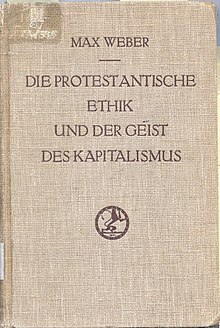
\includegraphics[width=\linewidth]{static/weber}
    \caption{Weber}
    \label{}
    \end{subfigure}
    \begin{subfigure}[b]{0.25\textwidth}
    \centering
    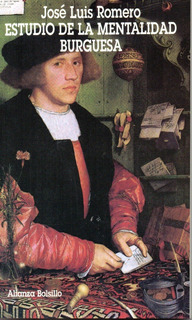
\includegraphics[width=0.9\linewidth]{static/romero}
    \caption{Romero}
    \label{}
    \end{subfigure}
    \begin{subfigure}[b]{0.25\textwidth}
    \centering
    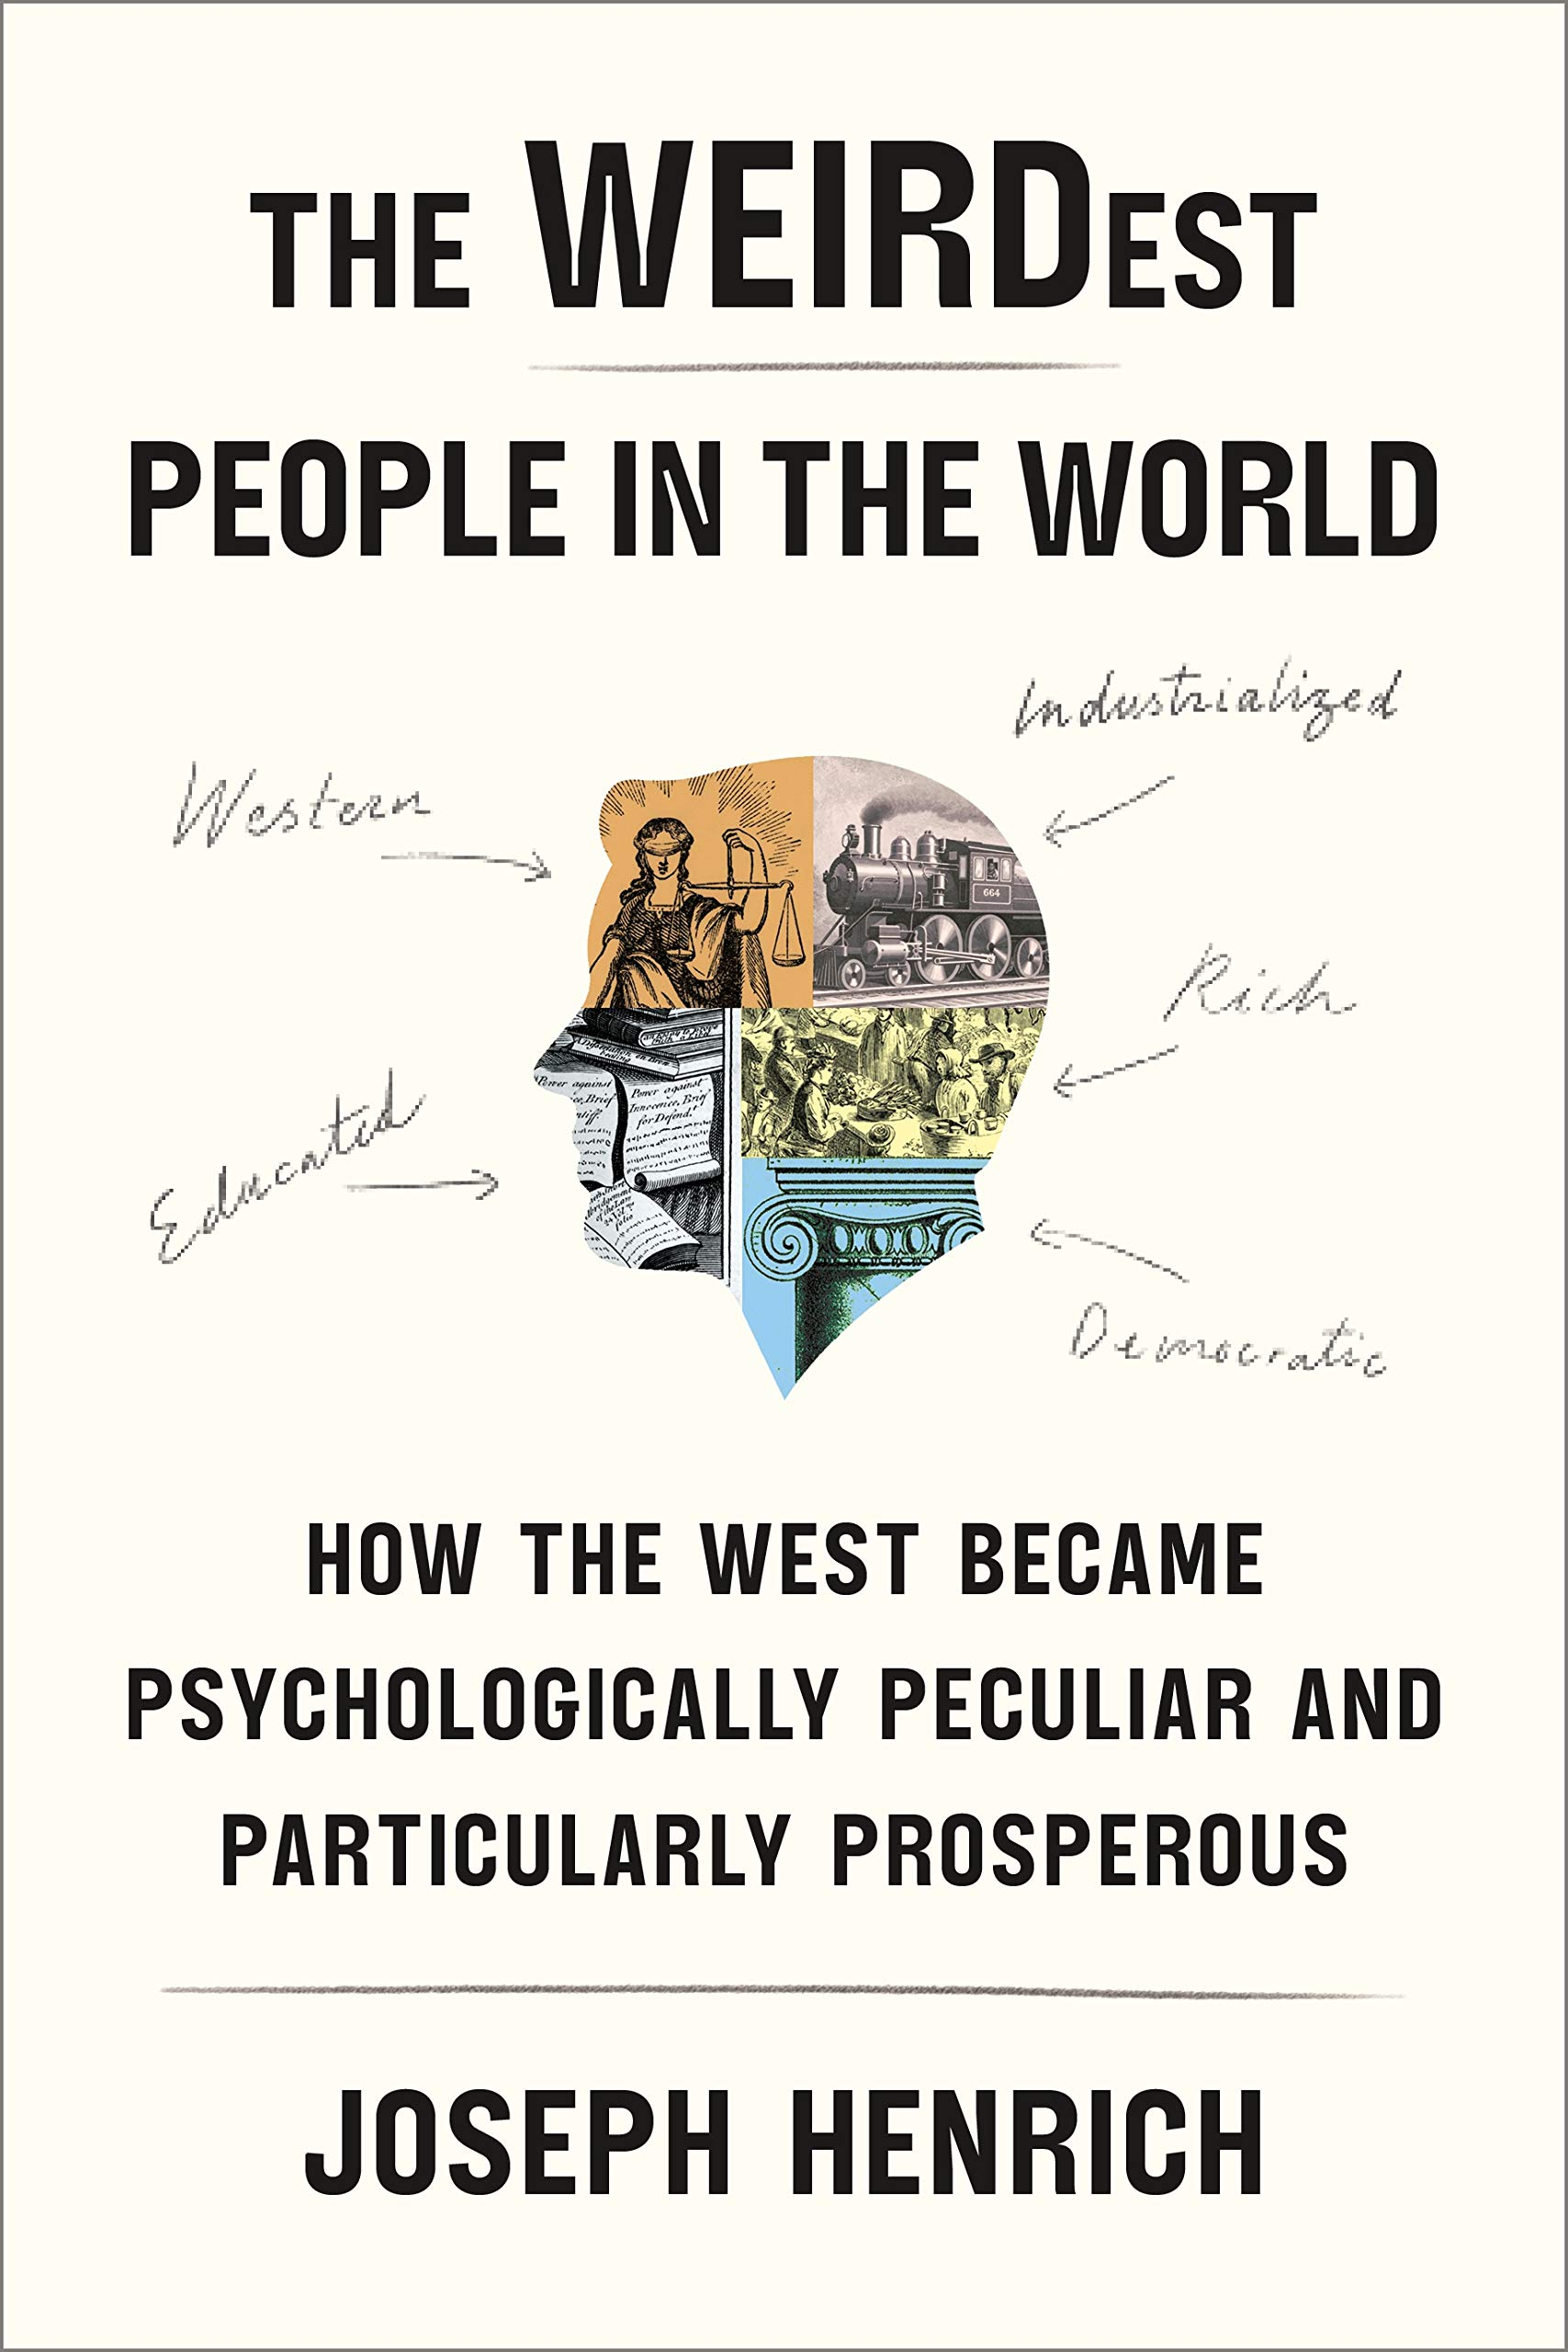
\includegraphics[width=1\linewidth]{static/henrich}
    \caption{Henrich}
    \label{}
    \end{subfigure}
    \caption{Mito eurocéntrico}
    \label{fig:mito}
\end{figure}

\es{El mito eurocéntrico proyecta a la europa feudal en la cultura griega y judeo-cristianismo (ambos fenómenos de origen oriental) con pretensión de explicación histórico-mundial: ``la historia universal va del Oriente al Occidente; Europa es el centro absoluto de la historia universal'' dice Hegel~\cite{hegel}.}%
%
\es{Este relato falso de la historia está vigente todavía en la principales univerisidades del mundo occidental, desde Harvard a la Universidas de Buenos Aires, pero también en universidades de África, del mundo Árabe, India y Asia.}%
%
\es{Desde Hegel hasta la fecha, las explicaciones eurocéntricas intentan explicar la proposperidad actual de occidente a través de una ``causa interna'': el ``espíritu protestante'' de Weber \cite{weber}, la ``mentalidad burguesa'' de Romero \cite{romero}, o más recientemente el ``sistema de parentezco''\cite{henrich} de Henrich.}%

% Parrafo

\es{La paradoja que no puede responder el relato eurocéntricos es cómo una sociedad sumida en un proceso de involución cultural como la sociedad feudal de la ``edad media'' puedo generar de repenten un proceso de desarrollo científico y técnico caracterísitico de la modernidad.}%
%
\es{Incluso Needham, el británico que recopiló la monumental historia científica y técnica de China, reconoce que comenzó a estudiar el tema motivado por responder la pregunta de por qué sólo europa había logrado el avance científico.}%
%
\begin{quotation}
When I first formed the idea, about 1938, (...) I regarded the essential problem as that of why modern science had not developed in Chinese civilisation (or Indian or Islamic) but only in that of Europe~\cite{needham2004-generalConclusionsAndReflections}.%
\end{quotation}
%
\es{Luego de 60 años de investigación Needham se ve obligado inviertir la pregunta.}%
%
\begin{quotation}
Why, between the -1th century and the 15th century, was Chinese civilisation much \emph{more} efficient than occidental in gaining natural knowledge and in applying it to practical human needs?~\cite{needham2004-generalConclusionsAndReflections}
\end{quotation}

%

\es{Ninguna de estas propuestas incorpora en su análisis la situación de aislamiento que sufre europa occidental en la etapa previa ni la situación de interconexión mundial posterior.}%
%
\es{La explicaciones de ``aislamiento e integración'' permiten explicar tanto el proceso de involución cultural que sufre la sociedad europea durante su ``edad media'' como la aceleración del proceso de evolución cultural que vive el mundo moderno.}%
%
\begin{figure}[ht!]
    \centering
    \begin{subfigure}[b]{0.25\textwidth}
    \centering
    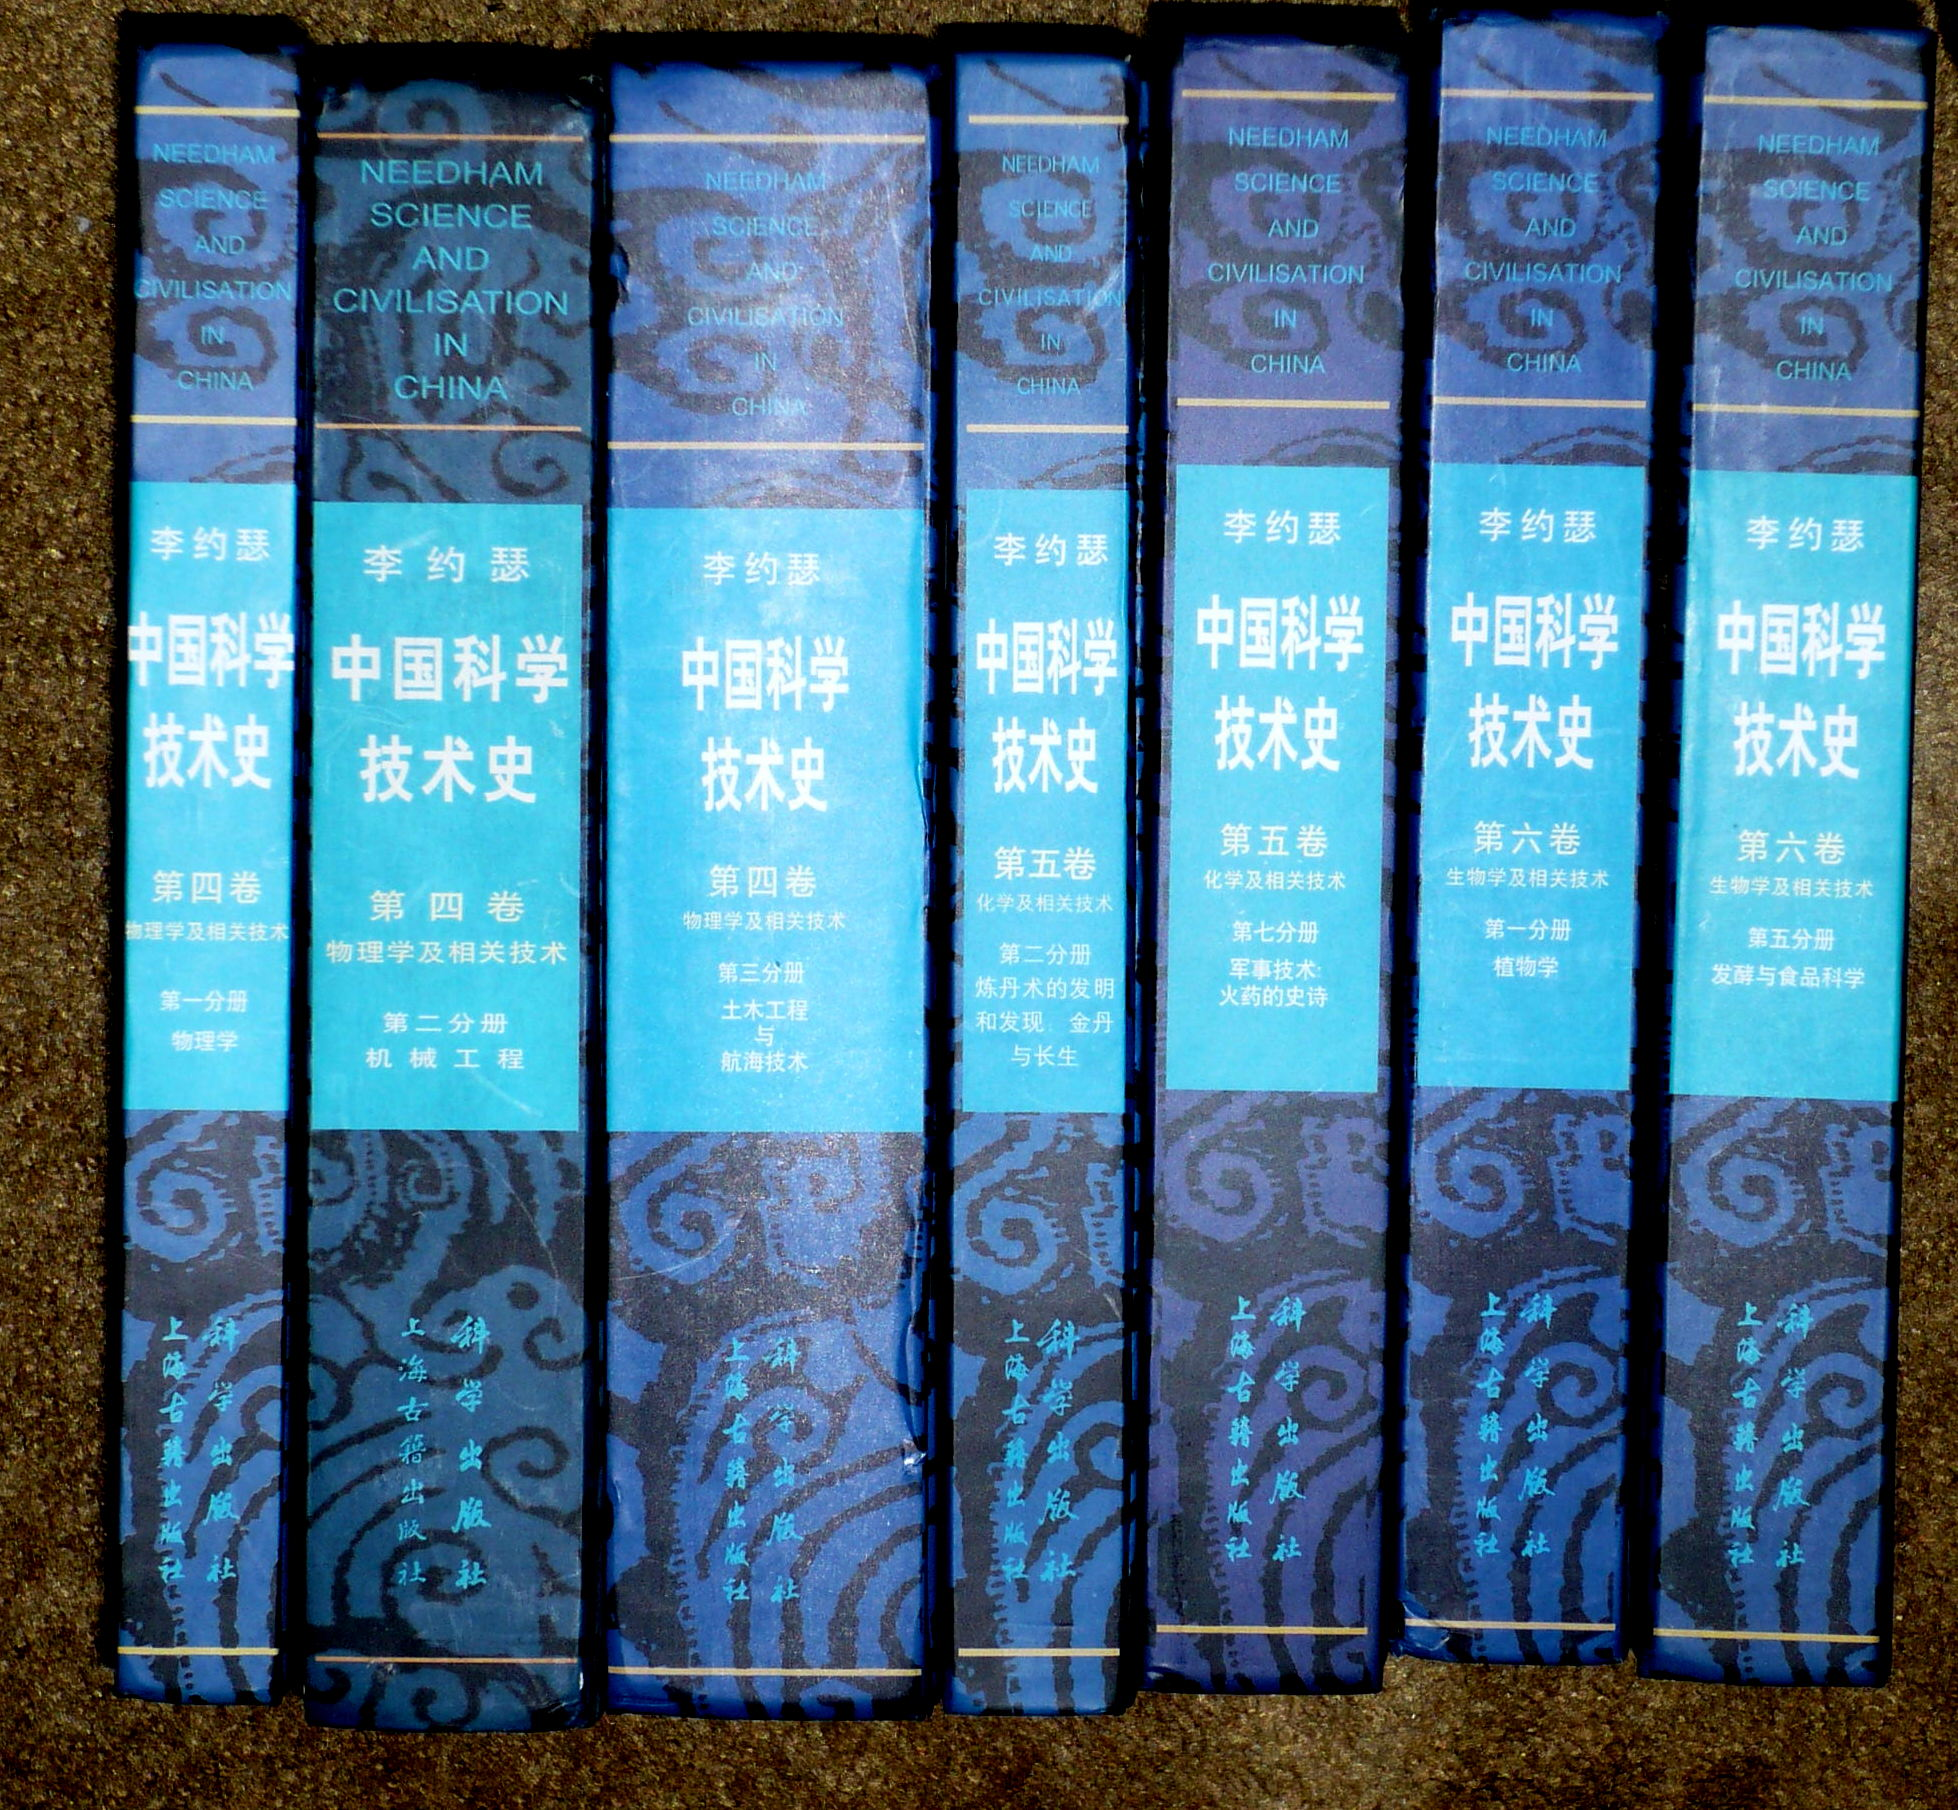
\includegraphics[width=\linewidth]{static/scienceAndCivilizationChina}
    \caption{Ciencia China}
    \label{}
    \end{subfigure}
    \begin{subfigure}[b]{0.35\textwidth}
    \centering
    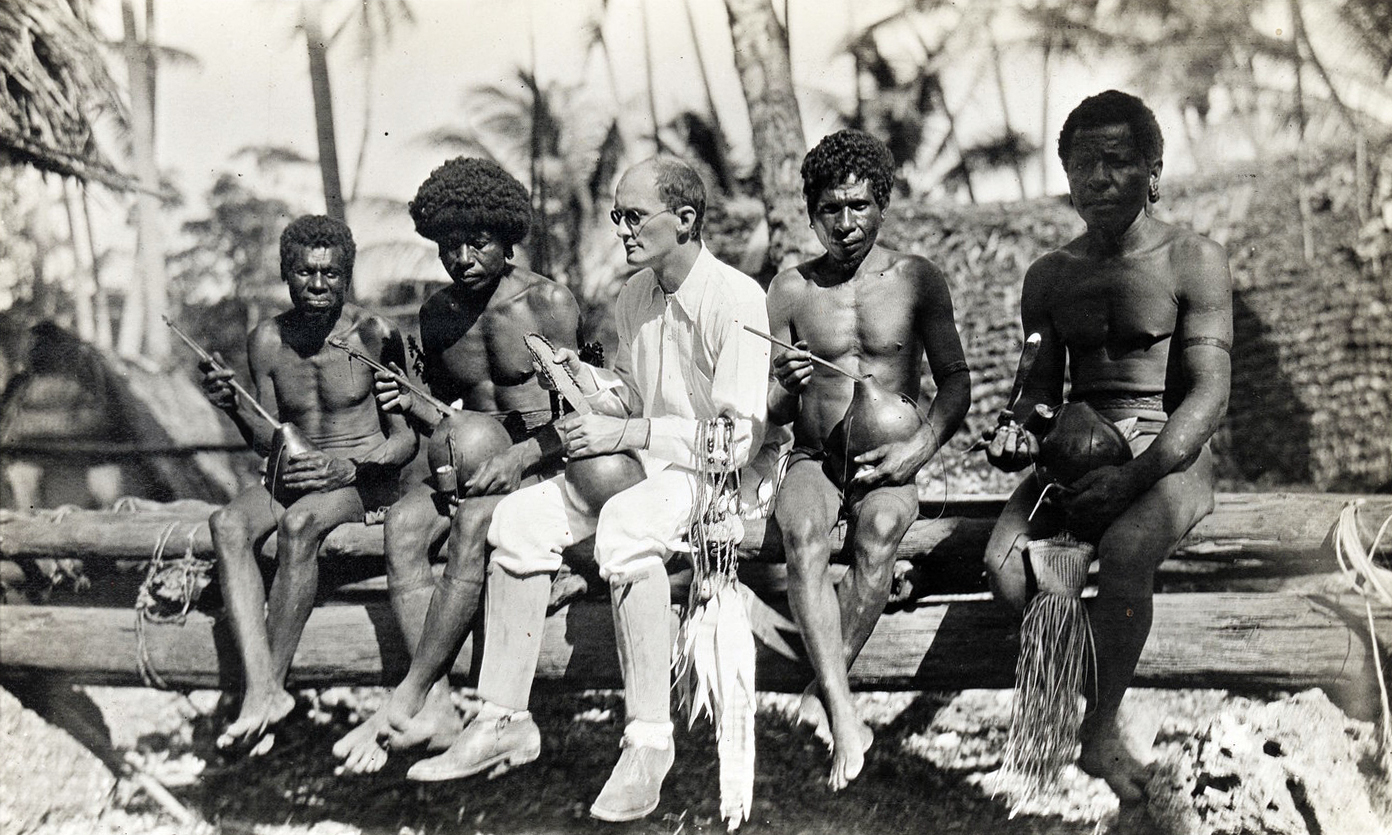
\includegraphics[width=\linewidth]{static/malinowsky}
    \caption{Ciencias locales}
    \label{}
    \end{subfigure}
    \caption{Hipótesis del ``aislamiento e integración''. Luego del aislamiento se produce una extraoirdinaria inegración con apropiación de los conocimientos mundiales.}
    \label{fig:mito}
\end{figure}
%
\es{Sin embargo, esta integración no estuvo impulsada solamente por los sucesos fortuitos que permitieron a una sociedad que escapaba de la violencia interna integrarse primero a américa gracias a la paz relativa de este continente y las epidemias que diesmaron su población, y luego a la plata americana que le permite a la europa occidental integrarse de repente a los sistemas de intercambio ya existentes en Africa, el mundo Árabe, India y China.}%
%
\es{La integración que permitió acelerar el proceso avance científico y técnico, estuvo acompañada también globalización de las tecnologías de colonización que la sociedad fedual había desarrollado durante su ``edad media'', y que fueron aplicadas a escala global desde entonces.}%
%
\es{Por eso, la explicación de ``aislamiento e integración'' permite explicar también el proceso de perdida de diversidad cultural ocurrida durante un proceso de integración que fue a su vez coloinal.}%
%
\es{La ``integración-colonial'' produjo un doble proceso, de avance cientítfico y tecnológico por un lado y de pérdida cultural por otro.}


\subsection{El criterio de acuerdos intersubjetivos y la adaptación ecológica}

\es{La crisis ecológica actual es producto del criterio de imposición colonial de la integración moderna: la ciencia metropolitana no es capaz de compensar la perdida de las conocimientos milenarios desarrollados por las comunidades autónomas locales.}
%
\es{Con la inflación del sujeto blanco-masculino, modelo de lo humano y de todo cuanto sea dotado de politicidad, interés general y valor universal, y la minorización del espacio de las mujeres y de los pueblos de todo el mundo, transformado en margen y resto de la política, la comunidades se debilitan internamente y pierden su autonomía.}
%
\en{In a world of uprooted individuals, the pedagogy of cruelty manages to introduce the typical psychopathic structure of our times based on instrumental desire and a worldview of things: nature as a thing, people as things.}%
\es{En un mundo de individuos desarraigados, la pedagogía de la crueldad consigue introducir la típica estructura psicopática de nuestro tiempo basada en el deseo instrumental y en una visión del mundo de las cosas: la naturaleza como cosa, las personas como cosas.}%
%
\es{Los conocimientos milenarios y sus instituciones adaptadas ecológicamente se pierden definitivamente en unas pocas generaciones.}%
%
\es{En un mundo de comunidades debilitadas, la pedagogía de la crueldad colonial consigue introducir la estructura psicopática típica de nuestro tiempo: el deseo individualista y una cosmovisión del mundo como cosa, la naturaleza como cosa, las personas como cosas.}%
%
% \es{Lo que debemos recuperar son las autonomías de los proyectos históricos comunitarios a través de las tecnologías de sociabilidad propias de la politicidad doméstica que las mujeres adminstraran en el espacio público del mundo aldea antes de que el patriarcado de alta intensidad de la colonial-modernidad las se transforma en margen y resto de la política.}%

%

\es{Even before the emergence of modern Homo sapiens, gender roles constitute the first social division of labor.}%
\es{Antes incluso de la aparición del Homo sapiens moderno, aparecen los roles de género como primera división social del trabajo.}%
%
\en{Biased by underlying sexual dimorphism, complementary cultural systems essential to the survival of communities evolved.}%
\es{Sesgados por el dimorfismo sexual subyacente, evolucionaron sistemas culturales complementarios esenciales para la supervivencia de las comunidades.}%
%
\en{Beyond cultural and prestige differences, the inter-community space, managed mainly by men, and the intra-community space, managed mainly by women, are in the pre-colonial world complementary activities with their own political competence.}%
\es{Más allá de las diferencias culturales y de prestigio, el espacio inter-comunitario, gestionado principalmente por los hombres, y el espacio intracomunitario, gestionado principalmente por las mujeres, son en el mundo precolonial actividades complementarias con estatus política y social propio.}%
%
\en{The hypothesis that patriarchy, or gender relations based on inequality, is the most archaic and permanent political structure of humanity is based on the existence of a mythical formula of planetary dispersion that relates a time when women were defeated and disciplined.}%
\es{La hipótesis de que el patriarcado, o las relaciones de género basadas en la desigualdad, es la estructura política más arcaica y permanente de la humanidad se basa en la existencia de una fórmula mítica de dispersión planetaria que relata una época en la que las mujeres fueron derrotadas y disciplinadas.}%
%
\es{La masculinidad, en todos los rincoones del planeta, es una posición que se adquiere mediante la exhibición púbica de poder - negociador, económico, sexual, moral, intelectual, bélico - y será nuevamente el punto débil de las comunidades, donde las tecnologías de colonización, desarrolladas por la sociedad fedual, actuan primero}


%
\en{Th structure of relationships is radically transformed in the colonial-modern transition: with the process of conquest and colonization, a low-intensity patriarchy of pre-colonial communities is transformed into a high-intensity patriarchy~\cite{paredes}.}%
\es{La estructura relaciones se transforma radicalmente en la transición colonial-moderna: con el proceso de conquista y colonización, el patriarcado de baja intensidad de las comunidades precoloniales se transforma en un patriarcado de alta intensidad~\cite{paredes}.}%


% Parrafo


% Parrafo 

\es{La Europa feudal no se había despertando del impacto de su invasión colonial cuando ya en 1514 Bartolomé de la Casas inicia desde América la advertencia de los efectos negativos de la integración basada en la dominación que ya promovían los primeros migrantes feudales.}%, tres años antes de que M. Lutero expusiera sus tesis en Erfurt o que Maquiavelo publicara Il Principe.
%
\es{En su crítica Bartolomé: a) refuta la pretensión de superioridad de la cultura occidental sobre las las culturas indígenas; b) diferencia entre otorgar al otro (al indio) pretensión universal de verdad, sin renunciar a la pretensión de predicar a favor la propia cultura cristiana; c) y demuestra la falsedad del el argumento usado para justificar la intervención en las autonomías locales, basado en la supuesta ``remedio a las injusticias internas'', en tanto esa intervenciones producían peores efectos sobre las poblaciones intervenidas.}%

%

\es{La defensa de las autonomías no se sustenta en argumentos relativistas, que reclaman el derecho de los pueblos a mantener su patrimonio cultural ancenstral.}
%
\es{El caso límite del infanticidio indígena nos enseña que, a pesar de que alla argumentos evolutivos para explicarlo, no es posible defender el derecho a la diferencia en un ambiente dominado por la episteme de la colonialidad y hegemonizado por el discurso de los derechos universales.}
%
\es{El abandono de las crías se observa casi exclusivamente en especies que, como la humana, requieren de la cooperación para proveer y cuidar a sus costosos jóvenes.}
%
\es{En la mayoría de las sociedades tradicionales de cazadores-recolectores, el abandono es poco frecuente y ocurre cuando la madre percibe que no recibirá el apoyo social necesario, sólo al instante posterior al parto.}%
%
\es{Si bien varias sociedades modernas garantizan la interrupción voluntaria del embarazo, es inviable la defensa de las autonomías a sociedades ya intervenidas si sus prácticas contradicen el marco normativo colonial-moderno en un campo tan sensible como los derechos de la infancia, siempre elegidos para afirmar la superioridad moral y el derecho la intervención civilizadora del colonizador.}%
%
\es{Este argumento culturalista es en si mismo un problema, en tanto limita el reconocimiento de los pueblos a la repetición esterotipada de ciertas prácticas que se consideran esenciales a su identidad.}%

% Parrafo

\es{La cultura sin embargo es un sistema de información trasgeneracional en permamente cambio.}%

\es{El derecho a las autonomías se sustenta en el hecho práctico de que el conocimiento cultural ecológicamente adaptado sólo evoluciona a través de la experiencia histórica que acumulan los pueblos\cite{Rita}.}%
%
\es{Lo que identifica a este sujeto colectivo, los pueblos, no es un patrimonio cultural estable, de contenidos fijos, sino la autopercepción por parte de sus miembros de compartir una historia común, que viene de un pasado y se dirige a un futuro, aun a través de situaciones de disenso interno y conflictividad.}
%
\es{Para promover nuevamente la evolución de instituciones adaptadas a los sistemas ecológicos se hace necesario restituir la jurisdicción y el fuero comunitario que permita a cada pueblo desplegar su propio proyecto histórico, un ``pluralismo histórico'' basado en las autonomías locales y una gobernanza poilicéntrica~\cite{Rita, Ostrom}.}%

%

\begin{figure}[ht!]
    \centering
    \begin{subfigure}[b]{0.45\textwidth}
    \centering
    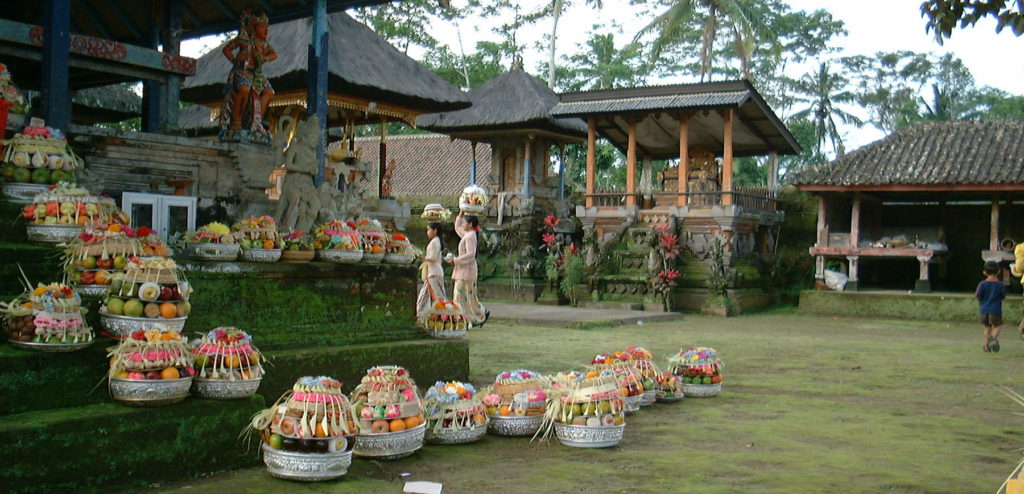
\includegraphics[width=\linewidth]{static/bali-offerings}
    \caption{Canang sari}
    \label{}
    \end{subfigure}
    \begin{subfigure}[b]{0.33\textwidth}
    \centering
    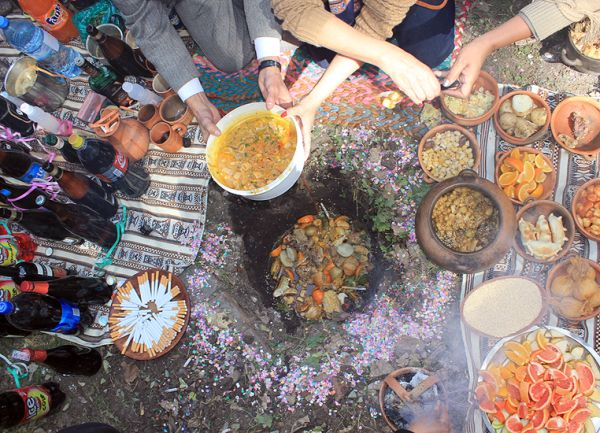
\includegraphics[width=\linewidth]{static/pachamama}
    \caption{Pachamama}
    \label{}
    \end{subfigure}
    \caption{La Madre Naturaleza como sujeto de derecho.}
    \label{fig:mito}
\end{figure}



\es{La intervención irracional de una especie sobre el sistema ecológico , que es el reservorio del único conocimiento adaptado para la vida, es la imposición total de la ignoracia sobre la verdad.}
%
\es{Para recuperar los conocimintos adaptados es necesario recuper el reconomineto mutuo perdido durante la modernidad.}
%
\es{Debemos obrar de una vez por todas ``de tal modo que la máxima de nuestra voluntad pueda valer siempre al mismo tiempo como principio de una legislación universal'', reconociendo esta vez como sujetos con valor universal a la universalidad toda: a las mujeres, jóvenes y adultos mayores de la propia comunidad, a los extranjeros y todos los miembros de los otros pubelos, a las otras especies, y a los sistemas ecológicos completos.}%
%
\es{Es la recuperación del estatus social y político de la politicidad doméstica adminstrada por principalmente por mujeres, el reconocimiento de los otros pueblos a tener autonomía histórica, pero también el derechos de la madre tierra (\emph{pachamama}) de no ver interrumpido sus procesos ecológicos sin justa causa: lo mínimo necesario para el buen vivir (\emph{suma kausay}).}%

%

\es{\textbf{El reconocmiento mutuo, que estuvo en la base de la evolución de nuestra especie, debe adquirir una universalidad plena para que valga como fundamento del conocimiento, que ni la propuesta parcial de Kant ni su cultura colonial ha sido capaz de alcanzar.}}


\section{Funciones como herramienta para los acuerdos intersubjetivos.}

El uso de funciones resulta inevitable en la construcción de conocimiento válido intersubjetivamente.
%
Su definición formal establece que una función es una relación (u operación) $f$ que a cada elemento de un conjunto (dominio) $X$ asigna un único elemento de otro conjunto (imagen) $Y$.
%
\begin{equation}
 \forall x \in X \  \exists! y \in Y \text{ tal que } f(x) = y    
\end{equation}
%
Esto se le como: ``para todo $x$ del dominio, existe un único $y$ de la imagen tal que $f(x)$ es igual a $y$''.
%
Visto sólo en términos formales, las funciones no parecen tener nada en especial respecto de otro tipo de relaciones posibles entre conjuntos.
%
Sin embargo lo que hace tan poderosa a las funciones es el hecho de que ellas permitan definir asignaciones no ambiguas.
%
El reconocmiento mutuo, sobre el que se base la fuente de validez del conocimiento, nos obliga a rechazar la superiordad moral o intelectual de subjetividades especiales o de grupos partículares (criterio de autoridad), en favor de criterios basados en la experiencia, definida como evidencia intelectual (universalidad y necesariedad por un lado) o evidencia sensible (fuente y acreditación empírica).
%
Para el proyecto intercultural de acuerdos intersubjetivos es fundamental poner en correspondencia unívoca los fenómenos percibidos por nuestras conciencias individuales con algún esquema de operación que sea públicamente inteligible y reproducible.
%
En este sentido, las funciones ocupan un rol fundamental.

\subsection{Los modelos causales deterministas como funciones teóricas}

La tendencia por entender el mundo en terminos de mecanismos ocultos de causa y efecto está extendida en todas las culturas.
%
Este idea todo lo que ocurre debe tener necesariamente una causa previa que lo genere se conoce en la historia de la filosofía como el pricipio de \emph{razón suficiente}.
%
El concepto de causa y efecto tiene nuevamete una estructura funcional, $f(x) = y$.
%
\begin{itemize}\setlength\itemsep{0cm}
 \item[$x$:] 
    {Condiciones iniciales (Causa)} 
 \item[$f$:] 
    {Modelo causal determinista (mecanismo subyacente)}
 \item[$y$:] 
    {Destino inevitable (efecto)}
\end{itemize}
%
Sin presencia de factores aleatorios, las condiciones iniciales del mundo determinan siempre el mismo destino inevitable.
%
Esta idea llevada al extremo, la de un mundo totalmente determinista, es rechazada tanto por experimentos de la física cuántica como por el supuesto teórico de libre albedrío de las ciencias sociales.
%
Sin embrago, los modelos causales deterministas se usan cotidianamente en todas las ramas de la ciencias empíricas para representar el funcionamiento del mundo, desde la física hasta las ciencias sociales.
%
Por ejemplo, en ajedrez Arpad Elo~\cite{ELO}, y otros antes de él, propusieron un modelo causal determinista en el que la habilidad y otros factores son la causa del resultado observado de la partida.
%
\begin{figure}[H]     
 \centering
  \tikz{         
    \node[det] (r) {$r$} ; 
    \node[const, left=of r, xshift=-2.35cm] (r_name) {\small \en{Result}\es{Ganar/perder}:}; 
    \node[const, right=of r] (dr) {\normalsize $ r = (d>0)$}; 

    \node[latent, above=of r, yshift=-0.45cm] (d) {$d$} ; %
    \node[const, right=of d] (dd) {\normalsize $ d=p_i-p_j$}; 
    \node[const, left=of d, xshift=-2.35cm] (s_name) {\small \en{Difference}\es{Diferencia}:};
    
    \node[latent, above=of d, xshift=-0.8cm, yshift=-0.45cm] (p1) {$p_i$} ; %
    \node[latent, above=of d, xshift=0.8cm, yshift=-0.45cm] (p2) {$p_j$} ; %
    \node[const, left=of p1, xshift=-1.55cm] (p_name) {\small \en{Performance}\es{Desempeño}:}; 

    \node[latent, above=of p1,yshift=0.7cm,fill=white] (s1) {$s_i$} ; %
    \node[latent, above=of p2,yshift=0.7cm,fill=white] (s2) {$s_j$} ; %
    
    \node[latent, above=of p1,xshift=-1cm, yshift=-0.45cm,fill=white] (u1) {$u_i$} ; 
    \node[latent, above=of p2,xshift=1cm, yshift=-0.45cm,fill=white] (u2) {$u_j$} ; 
    \node[const, left=of u1, xshift=-0.55cm] (u_name) {\small \en{Others factors}\es{Otros factores}:}; 
    
    \node[const, right=of p2] (dp2) {\normalsize $p = s + u$};

    \node[const, left=of s1, xshift=-1.55cm] (s_name) {\small \en{Skill}\es{Habilidad}:}; 
    
    \edge {d} {r};
    \edge {p1,p2} {d};
    \edge {s1} {p1};
    \edge {s2} {p2};
    \edge {u1} {p1};
    \edge {u2} {p2};
  }
  \caption{Modelos causal determinista en el que las habilidades y otros factores causan los resultados observables a través de la diferencia de rendimientos, $d=p_i-p_j$: quien haya obtenido mayor rendimiento gana, $r = (d > 0)$.
  Las flechas representan relaciones causales.
  Los círculos representan variables continuas, y los cuadrados variables discretas.}
  \label{fig:modelo_causal_deterministas}
\end{figure}
%
En la figura~\ref{fig:modelo_causal_deterministas} se propone una mecanismo oculto como explicación del resultado de la partidas.
%
Si el modelo fuera cierto y conociéramos con precisión tanto el valor de habilidad y de los otros factores involucrados durante cada partida, sabríamos quién ganaría en cada caso.
%
La variedad de comportamiento que puede adquirir este modelo es bastante reducida.
%
Ya veremos más adelante la utilidad que este tipo de modelos tiene para las ciencias empíricas y para la inferencia en particular.

% Parrafo

Los modelos causales deterministas son también la base de las ciencias formales.
%
En 2004 Matthew Cook demostró que un sistema unidimensional binario, con 8 reglas de actualización, puede ser tan complejos como una maquina de Turing \cite{cook2004-automata}.
%
\begin{figure}[ht!]
    \centering
    \includegraphics[width=0.4\linewidth]{static/rule110.png}
    \caption{Autómata celular propuesto por Stephen Wolfram, conocido como regla 110.}
    \label{fig:rule110}
\end{figure}
%
Este simple sistema tiene la complejidad necesaria para, en principio, ser capaz de computar lo mismo que cualquier computadora moderna.
%
Pero además, estos modelos deterministras puede desarrollar comportamientos de una complejidad tal que se vuelven impredecibles.
%
Para analizarlo, supongamos el siguiente modelo ``poblacional''.
%
El modelo establece que el tamaño de una población, medida como proporción respecto de la capacidad máxima de un sistema, depende exclusivamente de su tamaño en el tiempo anterior y de un factor de reproducción $r$. 
%
\begin{equation}
 \text{Población}(t+1) = r \cdot \text{Población}(t)\cdot (1-\text{Población}(t))
\end{equation}
% \tikz{         
%     \node[latent] (n1) {$x_t$} ; 
%     
%     \node[latent, right=of n1, xshift=3cm] (n2) {$x_{t+1}$} ;
%     
%      \path[->] (n1) edge node[yshift=0.25cm] {$rx_t(1-x_t)$} (n2);
% 
% }
%
Dependiendo del factor de reproducción y de la población inicial, vamos diferentes tipos de comportamiento.
%
En la figura~\ref{fig:poblacion} podemos ver tres comportamientos típicos.
%
\begin{figure}[ht!]
    \centering
    \begin{subfigure}[b]{0.32\textwidth}
    \includegraphics[page=3,width=\linewidth]{figures/poblacion.pdf}
    \caption{Punto fijo}
    \label{fig:poblacion_punto_fijo}
    \end{subfigure}
    \begin{subfigure}[b]{0.32\textwidth}
    \includegraphics[page=9,width=\linewidth]{figures/poblacion.pdf}
    \caption{Periódico}
    \label{fig:poblacion_periodico}
    \end{subfigure}
    \begin{subfigure}[b]{0.32\textwidth}
    \includegraphics[page=11,width=\linewidth]{figures/poblacion.pdf}
    \caption{Caótico}
    \label{fig:poblacion_caotico}
    \end{subfigure}
    \caption{
    Tipos de atractores del sistema a medida que aumentamos el valor del parámetro $r$
    }
    \label{fig:poblacion}
\end{figure}
%
Cuando el valor del parámetro $r$ es chico (figura~\ref{fig:poblacion_punto_fijo}) la población tiende a un valor fijo, sin importar el tamaño inicial de la población.
%
Cuando el valor del parámetro $r$ es intermedio (figura~\ref{fig:poblacion_periodico}) la población oscila en un período.
%
Cuando el valor del parámetro $r$ llega a su límite (figura~\ref{fig:poblacion_caotico}) la población tiene un comportamiento que parece caótico.
%
En la figura~\ref{fig:camino_al_caos} graficos como va ocurriendo el cambio a medida que cambiamos el parámetro $r$.
%
\begin{figure}[ht!]
    \centering
    \includegraphics[width=0.5\linewidth]{figures/camino_al_caos}
    \caption{Los puntos a los que converge el sistema luego de 1000 iteraciones temporales.}
    \label{fig:camino_al_caos}
\end{figure}
%
Una de las propiedades más interesantes del atractor caótico es la sensibilidad a las condiciones inciales.
%
Si hacemos zoom en los primeros 30 pasos temporales de la figura~\ref{fig:poblacion_caotico}, y observamos el comportamiento del sistema si modificamos levemente las condición inicial, veremos que rápidamente las historias divergen.
%
\begin{figure}[ht!]
    \centering
    \includegraphics[page=13,width=0.4\linewidth]{figures/poblacion}
    \caption{La linea negra comienza con una población de $0.5$ y la roja de $0.499$}
    \label{fig:sensibilidad}
\end{figure}
%
A pesar de que el modelo sea totalmente determinista, la sensibilidad a las condiciones iniciales impone un límite a la capacidad predicitiva.
%
En un sistema natural jamás podremos medir con infinitas precisión por lo que la simulación que se haga a partir de esos datos no servirá para predecir que ocurrirá con el sistema pasado los primeros pasos temporales.
%
Por más que la natrualeza sea determinista y conozcamos con perfecta precisión el mecanismo subyacente que determina el movimiento de cada partícula, si el sistema se encuentra en atractor caótico, jamás vamos a poder predecir el tiempo más allá de los primeros días.

\subsection{Las distribuciones de creencias como funciones de probabilidad}

 >Es posible crear números aleatorios?
 %
 El objetivo de crear números aleatorios nos impone la necesidad de crear una maquina no-funcional, que para una misma entrada $x$ la operación $f$ devuelva a veces un valor $y_1$ y a veces otro valor $y_2$. 
 %
 >Pero cómo podemos hacer para decidir cuándo devolever uno y cuando devolvemos otro sin niunguna otra información que $x$?
 %
 Parece que se nos impone al principio de razón suficiente, de que todo efecto necesita una causa que lo genere.
 %
 Y acá tenemos una única causa para generar dos efectos.
 
 % Parrafo
 
 Hasta ahora nadie a podido crear números aleatorios sin acudir a ``ruido natural''.
 %
 Todas las soluciones a este problema utilizan algún modelo determinista para generar secuencia de números que se ``asemejan'' a los números aleatorios.
 % 
 A pesar de que queramos librarnos de las funciones, ellas se novuelven.
 %
 En la sección anterior vimos como generar este tipo de comportamientos.
 %
 El modelo de poblaciones con $r = 3.99$ es un candidato interesante para simular números aleatorios.
 %
 En la figura~\ref{fig:pseudo_aleatorio} mostramos los primeros 2000 valores de esta función.
 %
 \begin{figure}[ht!]
    \centering
    \includegraphics[page=14,width=0.5\linewidth]{figures/poblacion}
    \caption{Generación de números pseudo aleatorios usando el modelo de poblaciones (Eq.\ref{}) con $r=3.99$.}
    \label{fig:sensibilidad}
 \end{figure}
 %
 Se puede ver que la secuencia de números todavía contiene algunos patrones que no cumplen con lo que esperamos de un número aleatorio.
 %
 Aunque podamos mejorar esto, es importante notar que esta secuencia de números, aunque se parezca, no es aleatoria.
 %
 Por el contrario, toda la secuencia está comprimida en el valor inicial y en la función, nada más distinto un número aleatorio.
 
 % Parrafo
 
 A pesar de que no se haya encontrado un método sistemático para la generación de números aleatorios, las ciencias físicas y las ciencias sociales afirman que el mundo no tiene forma de función.
 %
 Por ejemplo, en las ciencias sociales el concepto de libre albedrío afiirma que una persona expuesta ante un estado del universo $s$ tiene la capacidad de decidir tomar más de una acción $a_i$.
 %
 \begin{figure}[ht!]
\centering
    \scalebox{1}{
 \tikz{ %
        \node[estado] (s) {};
        \node[const, above=of s] {$s$};
        \node[accion, below=of s, xshift=-1cm] (a1) {} ; %
	\node[accion, below=of s, xshift=0cm] (a2) {} ; %
	\node[accion, below=of s, xshift=1cm] (a3) {} ; %
	\node[const, right=of a3] {$a$};
        \edge[-] {s} {a1,a2,a3};
      
	\node[estado, below=of a1,xshift=0cm] (s1a) {}; %
	  
	\node[estado, below=of a2,xshift=0cm] (s2a) {}; %
	   
	\node[estado, below=of a3,xshift=0cm] (s3a) {}; %
	    
	\node[const, right=of s3a] {$s^{\prime}$};
	\edge[-] {a1} {s1a};
	\edge[-] {a2} {s2a};
	\edge[-] {a3} {s3a};
        }
    
    }
    \caption{El concepto teórico libre albedrío afirma que una persona, ante un estados $s$ del universo, es capaz de elegir entre más de una acción $a_i$.}
    \label{fig:libre_albedrio}
\end{figure}
%
Sea porque el mundo natural admite la posibilidad de que un efecto surga sin su propia causa, o sea por nuestra incapacidad de reconocer el mundo en pleno detalle, situaciones como la descrita en la figura~\ref{fig:libre_albedrio} introducen incertidumbre.
%
Ya no es posible definir una función tal que dados los estados devuelva la acción, $f(s) = a_i$.
%
Sin embargo podemos expresar nuestra incertidumbre utilizando funciones, $P : \ \text{Acciones} \mapsto \mathbb{R}$.
%
Las funciones de probabilidad nos permiten inidicar nuestra ``distribución de creencias''.
%
En este caso sabemos, por ejemplo, que detrás de una de las siguientes cajas una persona escondió un regalo.
%
¿Pero dónde lo escondió?
%
\begin{figure}[H]     
 \centering
 \tikz{
    \node[factor, minimum size=0.8cm] (p1) {} ;
    \node[factor, minimum size=0.8cm, xshift=1.5cm] (p2) {} ;
    \node[factor, minimum size=0.8cm, xshift=3cm] (p3) {} ;
    
    \node[const, above=of p1, yshift=.15cm] (fp1) {$P(a_1)$};
    \node[const, above=of p2, yshift=.15cm] (fp2) {$P(a_2)$};
    \node[const, above=of p3, yshift=.15cm] (fp3) {$P(a_1)$};
    } 
 \caption{Información disponible: sabemos que hay un regalo detrás de sólo una de las tres cajas.}
 \label{fig:espacio_de_hipotesis}
\end{figure}
%
La figura~\ref{fig:espacio_de_hipotesis} nos ofrece suficiente información para definir un espacio de hipótesis: las tres cajas.
%
Sin embargo hay infinitas distribuciones de creencias posibles.
%
Por ejemplo, podemos tener el presentimiento de que está en la caja del medio.
%
En la figura \ref{fig:distribucion_de_creencias} mostramos dos posibles distribuciones de creencias que tienen preferencia esa caja.
%
\begin{figure}[H]     
 \centering
 \begin{subfigure}[b]{0.48\textwidth}
 \centering
  \tikz{ %
         \node[factor, minimum size=0.8cm] (p1) {} ;
         \node[factor, minimum size=0.8cm, xshift=1.5cm] (p2) {} ;
         \node[factor, minimum size=0.8cm, xshift=3cm] (p3) {} ;
         
         \node[const, above=of p1, yshift=.15cm] (fp1) {$0$};
         \node[const, above=of p2, yshift=.15cm] (fp2) {$1$};
         \node[const, above=of p3, yshift=.15cm] (fp3) {$0$};        
        }
    \caption{Preferencia total}
    \label{fig:preferencia_total}
 \end{subfigure}
 \begin{subfigure}[b]{0.48\textwidth}
 \centering
  \tikz{ %
         \node[factor, minimum size=0.8cm] (p1) {} ;
         \node[factor, minimum size=0.8cm, xshift=1.5cm] (p2) {} ;
         \node[factor, minimum size=0.8cm, xshift=3cm] (p3) {} ;
         
         \node[const, above=of p1, yshift=.15cm] (fp1) {$1/10$};
         \node[const, above=of p2, yshift=.15cm] (fp2) {$8/10$};
         \node[const, above=of p3, yshift=.15cm] (fp3) {$1/10$};        
        } 
    \caption{Preferencia parcial}
    \label{fig:preferencia_parcial}
 \end{subfigure}
\caption{Dos distribución de creencias que tienen preferencia por una de las hipótesis.}
 \label{fig:distribucion_de_creencias}
\end{figure}
%
La distribución de creencias de la figura~\ref{fig:preferencia_total} representa la certeza de que el regalo está en la caja del medio, mientras que la figura~\ref{fig:preferencia_parcial} representa sólo una preferencia que mantiene todavía cierta duda.
%
Pero si de verdad no tenemos ninguna información respecto de dónde está el regalo, ninguna de estas distribuciones parece ser una buena idea.
%
Más allá de los presentimientos personales de cada quién, podemos fácilmente llegar a un acuerdo respecto de que dada la información disponible hay motivos para tener preferencia por ninguna de las opciones.
%
En este caso, una distribución de creencias honesta sería repartir la creencia en partes iguales \ref{fig:distribucion_de_creencias_honesta}.
%
\begin{figure}[H]     
 \centering
\tikz{ %
        
         \node[factor, minimum size=.8cm] (p1) {} ;
         \node[factor, minimum size=.8cm, xshift=1.5cm] (p2) {} ;
         \node[factor, minimum size=.8cm, xshift=3cm] (p3) {} ;
         
         \node[const, above=of p1, yshift=.15cm] (fp1) {$1/3$};
         \node[const, above=of p2, yshift=.15cm] (fp2) {$1/3$};
         \node[const, above=of p3, yshift=.15cm] (fp3) {$1/3$};        
        } 
\caption{Distribución de creencias honesta cuando no tenemos información previa.}
 \label{fig:distribucion_de_creencias_honesta}
\end{figure}
%
Si llegamos a un acuerdo respecto de que no tenemos información previa, entonces estaremos de acuerdo en esta distribución de creencias.
%
Esta distribución de creencias que permite el acuerdo intersubjetivo la vamos a llamar creencia honesta.
%
Es interesante notar que la creencia honesta cuando no tenemos información previa es la que maximiza la incertidumbre, dividiendo la certidumbre en partes iguales.
%
Este se conoce como el \textbf{principio de indiferencia}.
%
% \begin{framed}
% \centering
%   Principio de indiferencia \\
% \textbf{Dividir las creencias en partes iguales}
% \end{framed}
%
En la sección~\ref{actualizacion} veremos cómo actualizar las creencias de forma honesta cuando recibimos nueva información, maximizando la incertidumbre dada los datos y modelos.

\subsection{Los datos como funciones empíricas}

Cada vez que hablamos del mundo, incluso de manera informal, estamos haciendo afirmaciones que tiene la estructura de una función.
%
Los datos pueden ser vistos como funciones empíricas, $f(x)=y$.
%
Mediante las ``funciones proposicionales'' podemos afirmar por ejemplo que la ideología del Partido Obrero es de izquierda, o que la habilidad de Maradona fue superior a la de Messi.
%
\begin{equation}\label{eq:opiniones}
 \emph{Ideología}(\text{Partido Obrero}) = \text{Izquierda} \  \ \ , \ \ \ \emph{Habilidad}(\text{Maradona}) > \emph{Habilidad}(\text{Messi})
\end{equation}
%
La función representa una cierta variable o característica, que aplicada sobre una cierta unidad de análisis devuelve un valor.
%
\begin{itemize}  \setlength\itemsep{0cm}
 \item[$x$] 
    \textbf{\en{Unit of analysis}\es{Unidad de análisis}} (UA)
 \item[$f$] 
   \en{\textbf{Variable} of the unit of analysis}
   \es{\textbf{Variable} de la unidad de análisis} (V)
 \item[$y$] 
   \en{\textbf{Value} of the variable}
   \es{\textbf{Resultado} o valor de la variable} (R)
\end{itemize}

Si bien proposiciones de la ecuación \ref{eq:opiniones} tienen una estructura funcional, al conversar informalmente no hacemos explícita la definición precisa de la función.
%
Ahí radica el origen de muchos de los desacuerdos que a veces tenemos cuando conversamos informalmente porque en general diferentes persona usan las mismas palabras para comunicar conceptos que en realidad son distintos.

%

El significado preciso del dato depende entonces de la operacionalización de la función. 
% 
Por este motivo Juan Samaja propone que la estructura de todo dato científico contiene un cuarto elemento: el esquema indicidor.
%
Todo esquema indicador se compone de dimensiones (D), que son especificaciones de la variable, y de procedimientos (P) protocolos, acciones a efectuar sobre cierta fuente de datos (F).
%
Las reacciones dan los indicadores (I), objetos perceptibles desde el sentido común, que interpretados constituyen los resultados (R).
%
Esta es la estructura invariante de todo dato (Hipótesis de Samaja).
%
\begin{table}[ht!]
\centering
\begin{tabular}{clcccc}
Resultado (R) & \multicolumn{1}{r|}{} &  & Variable (V) &  &  \multicolumn{1}{|c}{Unidad de Análisis (UA)} \\ \hline
   &  \multicolumn{1}{r|}{}    &  & Dimensiones (D) &  & \multicolumn{1}{|r}{} \\
                 Indicador (I)  &   & =  &  &  &  Fuente de datos (F) \\
 & \multicolumn{1}{r|}{} &  & Procedimientos (P) &        &    \multicolumn{1}{|r}{}  
\end{tabular}
\caption{}
\label{tab:matriz_datos}
\end{table}
%
El contenido de cada uno de sus elementos depende de una serie de supuestos.
%
La validez interna de un dato depende en gran medida de las dimensiones (D) elegidas, de que estas expresen fielmente el concepto de la variable, que expresen lo relevante de ella y sólo de ella, discriminado factores ajenos que puedan intervenir de manera no advertida.
%
El proceso de selección de las dimensiones de la variable, y el conjunto de hipótesis asociaciadas, se llama examen de \emph{representatividad}.
%
La etapa de identificación de la fuente de datos (F), que está basa en hipótesis acerca de la autenticidad y accesibilidad de la información, se conoce como examen de \emph{viabilidad}.
%
La confiabilidad del dato, por su parte, depende de que los procedimientos detecten sólo esa dimensión de la fuente y no otros estímulos asociados, y de discriminar mínimas cantidades.
%
La definición de los protocolos, y sus hipótesis, se denomina examen de \emph{confiabilidad}.
%
\begin{table}[ht!]
\centering
\begin{tabular}{clcccc}
¿Resultado? (R) & \multicolumn{1}{r|}{} &  & Habilidad (V) &  &  \multicolumn{1}{|c}{Tenistas (UA)} \\ \hline
   &  \multicolumn{1}{r|}{}    &  & Ganar/perder (D) &  & \multicolumn{1}{|r}{} \\
                 True/False (I)  &   & =  &  &  & \ \ \ \texttt{atptour.com} (F) \ \ \  \\
 & \multicolumn{1}{r|}{} &  & Scraper (P) &        &      \multicolumn{1}{|r}{}
\end{tabular}
\caption{}
\label{tab:operacionalizacion_habilidad}
\end{table}
%

Por ejemplo, basados en el modelos causal \ref{ELO-seccion determinista}, podemos utilizar los resultados de las partidas (ganar/perder) como una dimensión que especifica el concepto de la variable ``habilidad''.
%
Además, podemos utilizar la página oficial de la asociación de tenis profesional ATP, \texttt{atptout.com} como fuente de datos.
%
Por último, a través de un \emph{scraper} podemos extraer de forma segura los resultados de las partidas, generenado en cada caso un indicador binario (verdadero/falso).
%
Ahora bien, ¿cómo hacemos para pasar del indicador al resultado?.
%
Para ello necesitamos una última hipótesis: la hipótesis indiciadora.

%

La propuesta de Elo fue iniciar la variable habilidad con un valor arbitrario y actualizarla en base a la sorpresa.
%
Para computar la sorpresa, la solución de Elo se basa en un modelo causal determinista con incertidumbre: a diferencia del modelo anterior~\ref{} ahora el efecto de los otros factores desconocidos se modela con una distribución gaussiana.
%
\begin{figure}[H]     
 \centering
 \begin{subfigure}[c]{0.49\textwidth}    
   \tikz{         
    \node[det, fill=black!10] (r) {$r$} ; 
    \node[const, left=of r, xshift=-1.35cm] (r_name) {\small \en{Result}\es{Resultado}:}; 
    \node[const, right=of r] (dr) {\normalsize $ r = (d > 0)$}; 

    \node[latent, above=of r, yshift=-0.45cm] (d) {$d$} ; %
    \node[const, right=of d] (dd) {\normalsize $ d = p_i-p_j$}; 
    \node[const, left=of d, xshift=-1.35cm] (d_name) {\small \en{Difference}\es{Diferencia}:};
    
    \node[latent, above=of d, xshift=-0.8cm, yshift=-0.45cm] (p1) {$p_i$} ; %
    \node[latent, above=of d, xshift=0.8cm, yshift=-0.45cm] (p2) {$p_j$} ; %
    \node[const, left=of p1, xshift=-0.55cm] (p_name) {\small \en{Performance}\es{Desempeño}:}; 

    \node[accion, above=of p1,yshift=0.3cm] (s1) {} ; %
    \node[const, right=of s1] (ds1) {$s_i$};
    \node[accion, above=of p2,yshift=0.3cm] (s2) {} ; %
    \node[const, right=of s2] (ds2) {$s_j$};
    
    \node[const, right=of p2] (dp2) {\normalsize $p \sim \N(s,\beta^2)$};

    \node[const, left=of s1, xshift=-.85cm] (s_name) {\small \en{Skill}\es{Habilidad}:}; 
    
    \edge {d} {r};
    \edge {p1,p2} {d};
    \edge {s1} {p1};
    \edge {s2} {p2};
    %\node[invisible, right=of p2, xshift=4.35cm] (s-dist) {};
}
\end{subfigure}
   \begin{subfigure}[c]{0.49\textwidth}
       \includegraphics[width=0.8\textwidth]{figures/probaOfWin_2D.pdf} 
     \label{fig:probaOfWin_2D}
    \end{subfigure}
\caption{}
\label{fig:elo}
\end{figure}
%
Las estimaciones previas, el modelo y el dato inducen una predicción a priori.
%
%
Según el modelo, la probabilidad de ganar a priori, $P(r|s_i^{\text{old}},s_j^{\text{old}})$, es equivalemte a los volúmenes indicados en la figura \ref{fig:probaOfWin_2D}.
%
\begin{equation*}
 \Delta = \underbrace{(1 - P(r|s_i^{\text{old}},s_j^{\text{old}}))}_{\hfrac{\textbf{Sorpresa}}{\text{del resultado}}}
\end{equation*}
%
La idea es que la magnitud de la sorpresa $\Delta$ est\'a relacionada con cuan buenas son las estimaciones previas, y por lo tanto puede usarse para actualizarlas.
%
Resultados inesperados indicar\'ian que las estimaciones actuales no son del todo correctas y deber\'ian actualizarse en mayor medida que si hubieran ocurrido como se esperaba.
%
\begin{equation}\label{eq:elo_update}
 s_{\text{winner}_\text{new}} = s_{\text{winner}_\text{old}} + \Delta \ \ \ \ \ s_{\text{loser}_\text{new}} = s_{\text{loser}_\text{old}} - \Delta 
\end{equation}
%
Donde la sorpresa $\Delta$ act\'ua como factor de correcci\'on para ambas estimaciones previas.
%
Esta es la hipótesis indicadora de Elo.
%
Esta soluci\'on puede recuperar la escala relativa de los agentes, partiendo de valores iniciales arbitrarios.
%
\begin{center}
\tikz{ %
        \node[const] (e) {Estimaci\'on}; 

        \node[const, xshift=3cm] (p) {Predicci\'on};
        \node[const, xshift=1.5cm, yshift=-1cm] (s) {Sorpresa}; 
        
         \edge {e} {p};
         \edge {p} {s};
         \edge {s} {e};
} 
\end{center}
%
Sin embargo, tiene algunas debilidades por no tener en cuenta la incertidumbre sobre las estimaciones de los agentes, que veremos más adelante.


\section{Honestidad.}

% %
% La regla de actualizaci\'on (Ec.~\eqref{eq:elo_update}) es sim\'etrica, as\'i que lo que gana un agente el otro lo pierde.
% %
% Debido a que a los agentes nuevos comienzan con estimaciones arbitrarias (el mismo valor inicial para cualquier individuo), ellas tienden a generan alta sorpresa y por lo tanto pueden modificar bruscamente las estimaciones de sus oponentes a pesar de que ya hubieran convergido.
% %

Ahora una persona nos va a dar una pista.
Nos va a decir dónde no está el regalo.
Esta pista depende de dónde sí está el regalo.
En la figura \ref{fig:modelo_causal_base} mostramos la relación causal entre las variables.
\begin{figure}[H]     
 \centering
 \tikz{            
    \node[latent,] (r) {
\includegraphics[width=0.06\textwidth]{static/regalo.png}} ;
    \node[const,above=of r] (nr) {\Large $r$} ;    
    
    \node[latent, right=of r] (d) {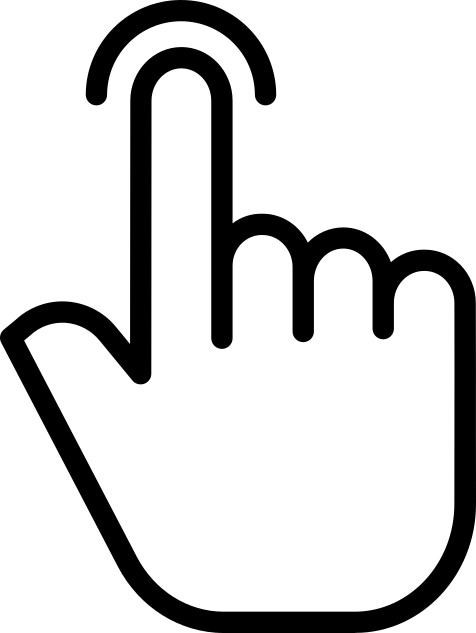
\includegraphics[width=0.05\textwidth]{static/dedo.png}};
    \node[const, above=of d] (nd) {\Large $s$} ;

    \edge {r} {d};
    }
  \caption{Las pistas dependen de dónde está el regalo.}
  \label{fig:modelo_causal_base}
\end{figure}

Ahora nuestra distribución de creencias no es sobre una variable, como hicimos antes, es sobre las dos variables.
\begin{equation}
 \text{Creencia}(r_i, s_j)
\end{equation}
Esto se lee como ``la creencia de que ocurran ambos: que el regalo esté en la cada $i$, $r_i$, y que la persona señale la caja $j$, $s_j$''.

\vspace{0.3cm}

Para determinar la creencia honesta en casos donde hay varias variables vinculadas por un modelo causal, sigue siendo necesario dividir la creencia en partes iguales, pero ahora por los caminos del modelo causal.


\begin{figure}[H]     
 \centering
    \tikz{
    \node[latent, draw=white, yshift=0.6cm] (b0) {$ 1$};

    \node[latent,below=of b0,yshift=0.6cm, xshift=-3cm] (r1) {$r_1$};
    \node[latent,below=of b0,yshift=0.6cm] (r2) {$r_2$};
    \node[latent,below=of b0,yshift=0.6cm, xshift=3cm] (r3) {$r_3$};

    \node[latent, below=of r1, draw=white, yshift=0.6cm] (br1) {$\frac{1}{3}$};
    \node[latent, below=of r2, draw=white, yshift=0.6cm] (br2) {$\frac{1}{3}$};
    \node[latent, below=of r3, draw=white, yshift=0.6cm] (br3) {$\frac{1}{3}$};

    \node[latent,below=of br1,yshift=0.6cm, xshift=-0.7cm] (r1d2) {$s_2$};
    \node[latent,below=of br1,yshift=0.6cm, xshift=0.7cm] (r1d3) {$s_3$};

    \node[latent,below=of r1d2,yshift=0.6cm,draw=white] (br1d2) {$\frac{1}{3}\frac{1}{2}$};
    \node[latent,below=of r1d3,yshift=0.6cm, draw=white] (br1d3) {$\frac{1}{3}\frac{1}{2}$};

    \node[latent,below=of br2,yshift=0.6cm, xshift=-0.7cm] (r2d1) {$s_1$};
    \node[latent,below=of br2,yshift=0.6cm, xshift=0.7cm] (r2d3) {$s_3$};
    \node[latent,below=of br3,yshift=0.6cm, xshift=-0.7cm] (r3d1) {$s_1$};
    \node[latent,below=of br3,yshift=0.6cm, xshift=0.7cm] (r3d2) {$s_2$};

    \node[latent,below=of r2d1,yshift=0.6cm, draw=white] (br2d1) {$\frac{1}{3}\frac{1}{2}$};
    \node[latent,below=of r2d3,yshift=0.6cm,draw=white] (br2d3) {$\frac{1}{3}\frac{1}{2}$};
    \node[latent,below=of r3d1,yshift=0.6cm, draw=white] (br3d1) {$\frac{1}{3}\frac{1}{2}$};
    \node[latent,below=of r3d2,yshift=0.6cm,draw=white] (br3d2) {$\frac{1}{3}\frac{1}{2}$};

    \edge[-] {b0} {r1,r2,r3};
    \edge[-] {r1} {br1};
    \edge[-] {r2} {br2};
    \edge[-] {r3} {br3};
    \edge[-] {br1} {r1d2,r1d3};
    \edge[-] {r1d2} {br1d2};
    \edge[-] {r1d3} {br1d3};
    \edge[-] {br2} {r2d1, r2d3};
    \edge[-] {br3} {r3d1,r3d2};
    \edge[-] {r2d1} {br2d1};
    \edge[-] {r2d3} {br2d3};
    \edge[-] {r3d1} {br3d1};
    \edge[-] {r3d2} {br3d2};
    }
  \caption{Dividir las creencias en partes iguales por los caminos del modelo causal}
  \label{fig:dividir_creencias_modelo_causal}
\end{figure}

Esto nos determina la distribución de creencias conjunta honesta.
Decimos conjunta porque estamos hablando de creencias sobre más de una variable a la vez.
La tabla \ref{tab:creencia_conjunta_honesta} la completamos con las creencias que tienen los caminos en la figura \ref{fig:dividir_creencias_modelo_causal}.
\begin{table}[H]
  \centering
  Creencia$(r,s)$ \\ \vspace{0.3cm}
 \begin{tabular}{c|c|c|c|} \setlength\tabcolsep{0.4cm} 
        & \, $r_1$ \, &  \, $r_2$ \, & \, $r_3$ \, \\ \hline 
  $s_1$  & $0$ & $1/6$ & $1/6$  \\ \hline
  $s_2$  & $1/6$ & $0$ & $1/6$   \\ \hline
       $s_3$ & $1/6$ & $1/6$ & $0$   \\ \hline 
\end{tabular}
\caption{Distribución de creencias conjunta honesta}
\label{tab:creencia_conjunta_honesta}
\end{table}

Conseguimos la distribución de creencias de que ocurran ambas cosas a la vez.
¿Cuál es la creencia de que el regalo esté en las cajas?
\begin{equation}
 \text{Creencia}(r_i)
\end{equation}

\todo[inline, color=gray!50]{Explicar esto primero de forma intuitiva. Vas a estar introduciendo la regla de la suma.}

Finalmente, en la tabla \ref{tab:creencia_marginal_honesta} mostramos el resultado de integrar las creencias conjunta para obtener la creencia de una única variable.
\begin{table}[H]
  \centering
    Creencia$(r,s)$ \\ \vspace{0.3cm}
    \begin{tabular}{c|c|c|c||c} \setlength\tabcolsep{0.4cm} 
            & \, $r_1$ \, &  \, $r_2$ \, & \, $r_3$ \, & \phantom{\bm{$1/3$}} \\ \hline 
    $s_1$ & $0$ & $1/6$ & $1/6$ & $1/3$ \\ \hline
    $s_2$ & $1/6$ & $0$ & $1/6$ & $1/3$ \\ \hline
    $s_3$ & $1/6$ & $1/6$ & $0$ & $1/3$ \\ \hline \hline
            & $1/3$ & $1/3$ & $1/3$ & $1$ \\ 
    \end{tabular}
  \caption{Integrar creencias.}
  \label{tab:creencia_marginal_honesta}
\end{table}

\begin{framed} \centering
Regla 1 \\
\textbf{Integrar las creencias en partes iguales}
\end{framed}

En términos formales esto no es más que sumar todos los términos de la conjunta.
\begin{equation*}
\text{Creencia}(r_i) = \sum_j \text{Creencia}(r_i, s_j) 
\end{equation*}

\todo[inline, color=gray!50]{expicar esta función, cómo se lee la sumatoria, que signific el subíndice de la sumatoria, etc}

\section{Las reglas de la honestidad (o actualización de creencias)}

Ya sabemos como definir distribución de creencias honestas cuando no tenemos información.
Ahora, ¿cómo se actualizan las distribución de creencia de forma honesta luego de obtener información nueva?
Por ejemplo, si no ponemos en duda que la pista del que nos dan depende de las relación causal expuesta en la figura \ref{fig:modelo_causal_base}, ¿cuál es la forma honesta de actualizar creencias?

\begin{figure}[H]
\centering
 \tikz{ %
        
         \node[factor, minimum size=1cm] (p1) {} ;
         \node[det, minimum size=1cm, xshift=1.5cm] (p2) {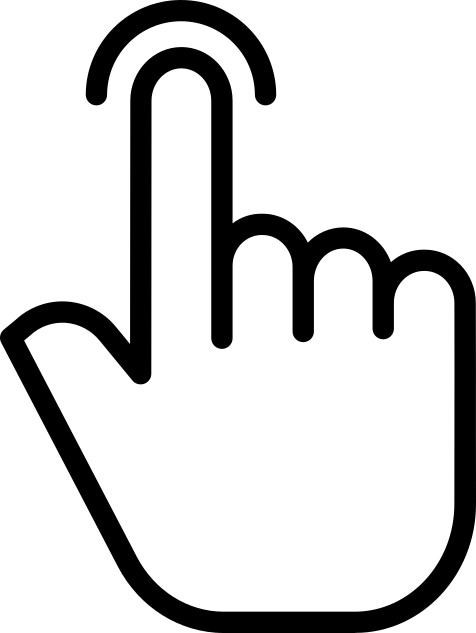
\includegraphics[width=0.03\textwidth]{static/dedo.png}} ;
         \node[factor, minimum size=1cm, xshift=3cm] (p3) {} ;

         \node[const, above=of p1, yshift=.15cm] (fp1) {$?$};
         \node[const, above=of p2, yshift=.15cm] (fp2) {$0$};
         \node[const, above=of p3, yshift=.15cm] (fp3) {$?$};
         \node[const, below=of p2, yshift=-.10cm, xshift=0.3cm] (dedo) {};
        } 
 \caption{Recibimos una pista que nos dice dónde no está el regalo.}
 \label{fig:pista_no_regalo}
\end{figure}

Si ya tenemos una creencia honesta previa, y ahora vemos un dato, lo que podemos hacer es quedarnos con la creencia previa que es compatible con el dato.
El resto fue creencia que asignamos opciones que ya no son compatibles con la realidad, el dato. 

\begin{table}[H]
\centering
Creencia$(r,s_2)$ \\ \vspace{0.3cm}
 \begin{tabular}{c|c|c|c||c} \setlength\tabcolsep{0.4cm} 
        & \, $r_1$ \, &  \, $r_2$ \, & \, $r_3$ \, &  \phantom{\bm{$1/3$}} \\ \hline 
  &  &  &  & \\ \hline
  $s_2$ & $1/6$ & $0$ & $1/6$ & $1/3$\\ \hline
  &  &  & &  \\ 
\end{tabular}
\caption{Creencias conjunta honestas compatible con el dato}
\label{tab:creencia_condicional_proporcional}
\end{table}

De la creencia conjunta honesta, solo sobrevive aquella que es compatible con el dato, que la pista fue la puerta 2.
 
\vspace{0.3cm}

Después de haber visto los datos, la creencia total se redujo a $1/3$.
Pero si esta es ahora nuestra creencia total, quisieramos volver a expresarla como $1$, en el sentido de que representa el $100$\% de nuestras creencias actuales.
Esto se logra normalizando, dividiendo por la creencia total que nos quedó $1/3$.
\begin{table}[H]
\centering
Creencia$(r|s_2)$ \\ \vspace{0.3cm}
 \begin{tabular}{c|c|c|c||c} \setlength\tabcolsep{0.4cm} 
        & \, $r_1$ \, &  \, $r_2$ \, & \, $r_3$ \, &  \phantom{\bm{$1/3$}} \\ \hline 
  &  &  &  & \\ \hline
  $s_2$ & $1/2$ & $0$ & $1/2$ & $1$ \\ \hline
  &  &  & &  \\ 
\end{tabular}
\caption{Creencia condicional}
\label{tab:creencia_condicional}
\end{table}

Es decir, a partir de la creencia honesta inicial y la pista podemos decir que la creencia honesta actualizada en este caso es
\begin{figure}[H]
 \centering
\tikz{ %
        
         \node[factor, minimum size=1cm] (p1) {} ;
         \node[det, minimum size=1cm, xshift=1.5cm] (p2) {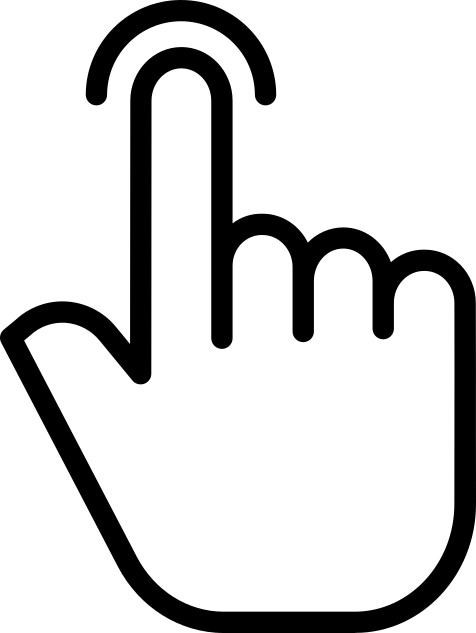
\includegraphics[width=0.03\textwidth]{static/dedo.png}} ;
         \node[factor, minimum size=1cm, xshift=3cm] (p3) {} ;

         \node[const, above=of p1, yshift=.15cm] (fp1) {$1/2$};
         \node[const, above=of p2, yshift=.15cm] (fp2) {$0$};
         \node[const, above=of p3, yshift=.15cm] (fp3) {$1/2$};
         \node[const, below=of p2, yshift=-.10cm, xshift=0.3cm] (dedo) {};
        
        } 
\caption{Creencia actualizada.}
\label{fig:creencia_condicional}
\end{figure}

\begin{framed} \centering
  Regla 2 \\
\textbf{Contextualizar las creencias en partes iguales} 
\end{framed}

\begin{align*}
 P(r|s_2) = \frac{P(r, s_2)}{P(s_2)}
 \end{align*} 
 
 \todo[inline, color=gray!50]{Explicar esta función.}


\section{Las reglas de la probabilidad}

\begin{equation*}
  \text{Marginal}_{i} = \sum_j \text{Conjunta}_{ij}  \ \ \ \ \ \ \ \ \  \ \ \ \ \ \ \ \ \ \ \ \ \ \ \  \text{Condicional}_{j|i} = \frac{\text{Conjunta}_{ij}}{\text{Marginal}_{i}}
\end{equation*}

\todo[inline, color=gray!50]{Volver a hablar de las regla 1 (integrar creencias) y de la regla 2 (contextualizar creencias).}

\begin{equation}\tag{\text{Regla de la suma}}
 P(r) = \sum_j P(r,s_j)
\end{equation}
Cualquier distribución marginal puede ser obtenida integrando la distribución conjunta

\begin{equation}\tag{\text{Regla del producto}}
 P(r,s) = P(s|r)P(r)
\end{equation}
Cualquier distribución conjunta puede ser expresada como el producto de distribuciones condicionales uni-dimensionles.

\vspace{0.3cm}

El teorema de Cox \cite{citar biblio} dice que estas reglas que las encontramos intuitivamente son las únicas reglas que grantizan:
\begin{itemize} \setlength\itemsep{0cm}
 \item[$\bullet$] Representar las creencias con valores reales 
 \item[$\bullet$] Actualizar las creencias en la direcci\'on de la evidencia
 \item[$\bullet$] Consistencia, todos los caminos conducen a la misma conslusión
 \end{itemize}
 
Es decir, estas reglas no son reglas arbitrarias.
Son las reglas óptimas en el sentido de la honestidad, utilizan toda la información disponible, ni más ni menos, por lo que son de validez intercultural.

\vspace{0.3cm}

\todo[inline, color=gray!50]{Escribir mejor la conlusión interculutral, las consecuencias de que sean reglas honestas y teóricamente las únicas posibles}

In 1946, thanks to Cox, it was now a theorem that any set of rules for conducting inference, in which we represent degrees of plausibility by real numbers, is necessarily either equivalent to the Laplace-Jefreys rules, or inconsistent
 
\section{Monty Hall}

\todo[inline, color=gray!50]{Explicar monty hall}

\begin{figure}[H]
\centering
\tikz{        
    
    \node[latent] (d) {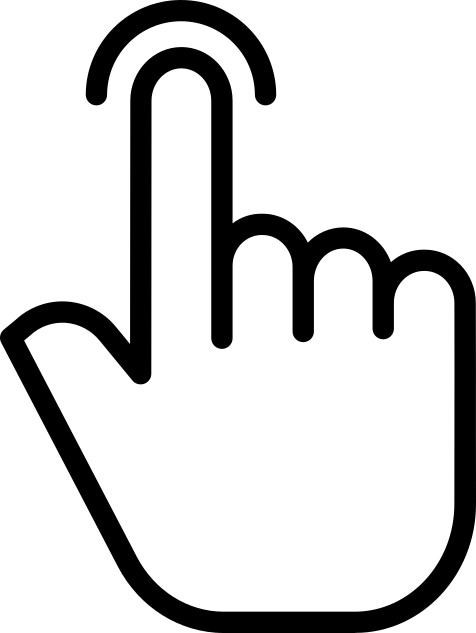
\includegraphics[width=0.05\textwidth]{static/dedo.png}} ;
    \node[const,above=of d] (nd) {\Large $s$} ;
    
    \node[latent, above=of d, xshift=-1.5cm] (r) {
\includegraphics[width=0.06\textwidth]{static/regalo.png}} ;
    \node[const,above=of r] (nr) {\Large $r$} ;
    
    \node[latent, fill=black!30, above=of d, xshift=1.5cm] (c) {
\includegraphics[width=0.06\textwidth]{static/cerradura.png}} ;
    \node[const,above=of c] (nc) {\Large $c$} ;
    
    \edge {r,c} {d};
}
\caption{Monty Hall}
\label{fig:modelo_monty_hall}
\end{figure}

Escribir ...


\begin{figure}[H]
\centering
\tikz{ %
         \node[factor, minimum size=1cm] (p1) {} ;
         \node[factor, minimum size=1cm, xshift=1.5cm] (p2) {} ;
         \node[factor, minimum size=1cm, xshift=3cm] (p3) {} ;

         \node[const, above=of p1, yshift=.15cm] (fp1) {$1/3$};
         \node[const, above=of p2, yshift=.15cm] (fp2) {$1/3$};
         \node[const, above=of p3, yshift=.15cm] (fp3) {$1/3$};
        
        } 
\caption{Escribir ...}
\label{fig:monty_hall_regalo}
\end{figure}

Escribir ...

\begin{figure}[H]
\centering
\tikz{ %
         \node[factor, minimum size=1cm] (p1) {
\includegraphics[width=0.025\textwidth]{static/cerradura.png}} ;
         \node[factor, minimum size=1cm, xshift=1.5cm] (p2) {} ;
         \node[factor, minimum size=1cm, xshift=3cm] (p3) {} ;

         \node[const, above=of p1, yshift=.15cm] (fp1) {$1/3$};
         \node[const, above=of p2, yshift=.15cm] (fp2) {$1/3$};
         \node[const, above=of p3, yshift=.15cm] (fp3) {$1/3$};
        
        } 
\caption{Escribir ...}
\label{fig:monty_hall_cerradura}
\end{figure}

Escribir ...

\begin{figure}[H]
 \centering
\tikz{ %
        
         \node[factor, minimum size=1cm] (p1) {
\includegraphics[width=0.025\textwidth]{static/cerradura.png}} ;
         \node[det, minimum size=1cm, xshift=1.5cm] (p2) {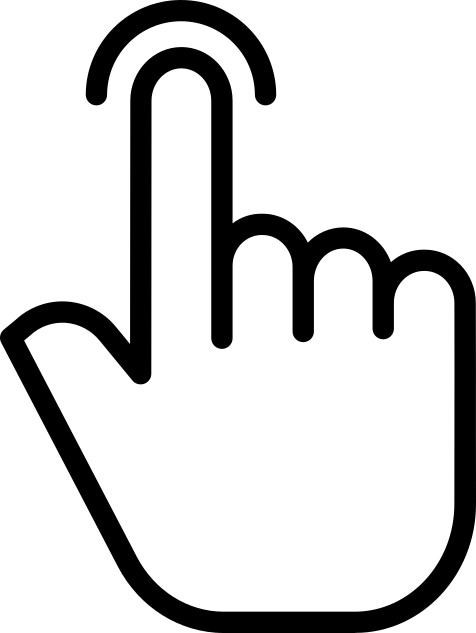
\includegraphics[width=0.03\textwidth]{static/dedo.png}} ;
         \node[factor, minimum size=1cm, xshift=3cm] (p3) {} ;
         
         \node[const, above=of p1, yshift=.15cm] (fp1) {$?$};
         \node[const, above=of p2, yshift=.15cm] (fp2) {$0$};
         \node[const, above=of p3, yshift=.15cm] (fp3) {$?$};
         \node[const, below=of p2, yshift=-.10cm, xshift=0.3cm] (dedo) {};
        
        } 
\caption{Escribir ...}
\label{fig:monty_hall_pista}
\end{figure}

Escribir ...


\begin{figure}[H]
\centering
\tikz{
\node[latent, draw=white, yshift=0.8cm] (b0) {$1$};
\node[latent,below=of b0,yshift=0.8cm, xshift=-2cm] (r1) {$r_1$};
\node[latent,below=of b0,yshift=0.8cm] (r2) {$r_2$};
\node[latent,below=of b0,yshift=0.8cm, xshift=2cm] (r3) {$r_3$};

\node[latent, below=of r1, draw=white, yshift=0.8cm] (br1) {$\frac{1}{3}$};
\node[latent, below=of r2, draw=white, yshift=0.8cm] (br2) {$\frac{1}{3}$};
\node[latent, below=of r3, draw=white, yshift=0.8cm] (br3) {$\frac{1}{3}$};

\node[latent,below=of br1,yshift=0.8cm] (c11) {$c_1$};
\node[latent,below=of br2,yshift=0.8cm] (c12) {$c_1$};
\node[latent,below=of br3,yshift=0.8cm] (c13) {$c_1$};

\node[latent, below=of c11, draw=white, yshift=0.8cm] (bc11) {$\frac{1}{3}$};
\node[latent, below=of c12, draw=white, yshift=0.8cm] (bc12) {$\frac{1}{3}$};
\node[latent, below=of c13, draw=white, yshift=0.8cm] (bc13) {$\frac{1}{3}$};

\node[latent,below=of bc11,yshift=0.8cm, xshift=-0.7cm] (r1d2) {$s_2$};
\node[latent,below=of bc11,yshift=0.8cm, xshift=0.7cm] (r1d3) {$s_3$};
\node[latent,below=of bc12,yshift=0.8cm] (r2d3) {$s_3$};
\node[latent,below=of bc13,yshift=0.8cm] (r3d2) {$s_2$};

\node[latent,below=of r1d2,yshift=0.8cm,draw=white] (br1d2) {$\frac{1}{3}\frac{1}{2}$};
\node[latent,below=of r1d3,yshift=0.8cm, draw=white] (br1d3) {$\frac{1}{3}\frac{1}{2}$};
\node[latent,below=of r2d3,yshift=0.8cm,draw=white] (br2d3) {$\frac{1}{3}$};
\node[latent,below=of r3d2,yshift=0.8cm,draw=white] (br3d2) {$\frac{1}{3}$};

\edge[-] {b0} {r1,r2,r3};
\edge[-] {r1} {br1};
\edge[-] {r2} {br2};
\edge[-] {r3} {br3};
\edge[-] {br1} {c11};
\edge[-] {br2} {c12};
\edge[-] {br3} {c13};
\edge[-] {c11} {bc11};
\edge[-] {c12} {bc12};
\edge[-] {c13} {bc13};
\edge[-] {bc11} {r1d2,r1d3};
\edge[-] {bc12} {r2d3};
\edge[-] {bc13} {r3d2};
\edge[-] {r1d2} {br1d2};
\edge[-] {r1d3} {br1d3};
\edge[-] {r2d3} {br2d3};
\edge[-] {r3d2} {br3d2};
}
\caption{}
\label{fig:monty_hall_caminos}
\end{figure}

Escribir ...

\begin{table}[H]
\centering
$P(r,s)$ \\ \vspace{0.3cm}
 \begin{tabular}{c|c|c|c|} \setlength\tabcolsep{0.4cm} 
        & \, $r_1$ \, &  \, $r_2$ \, & \, $r_3$ \, \\ \hline 
  { $s_2$}  & {$1/6$} & {$0$} & {$1/3$} \\ \hline
       {$s_3$} & {$1/6$} & {$1/3$} & {$0$}  \\ \hline
    \end{tabular}
\caption{Escribir ...}
\label{tab:monty_hall_conjunta}
\end{table}

Escribir ...

\begin{table}[H]
\centering
$P(r,s)$ \\ \vspace{0.3cm}
 \begin{tabular}{c|c|c|c||c} \setlength\tabcolsep{0.4cm} 
        & \, $r_1$ \, &  \, $r_2$ \, & \, $r_3$ \, & \\ \hline 
  { $s_2$}  & {$1/6$} & {$0$} & {$1/3$} & {$1/2$} \\ \hline
       {$s_3$} & {$1/6$} & {$1/3$} & {$0$} & {$1/2$} \\ \hline
              & {$1/3$} & {$1/3$} & {$1/3$}  & {$1$} \\ 
\end{tabular}
\caption{Escribir ...}
\label{tab:monty_hall_conjunta_y_marginal}
\end{table}

Escribir ...

\begin{table}[H]
 \centering
$P(r,s_2)$ \\ \vspace{0.3cm}
 \begin{tabular}{c|c|c|c||c} \setlength\tabcolsep{0.4cm} 
        & \, $r_1$ \, &  \, $r_2$ \, & \, $r_3$ \, & \\ \hline 
        { $s_2$}  & {$1/6$} & {$0$} & {$1/3$} & {$1/2$} \\ \hline
\end{tabular}
\caption{}
\label{tab:monty_hall_conjunta_compatible}
\end{table}

Escribir ...

\begin{table}[H]
 \centering
$P(r|s_2)$ \\ \vspace{0.3cm}
 \begin{tabular}{c|c|c|c||c} \setlength\tabcolsep{0.4cm} 
        & \, $r_1$ \, &  \, $r_2$ \, & \, $r_3$ \, & \phantom{$1/2$}\\ \hline 
  { $s_2$}  & {$1/3$} & {$0$} & {$2/3$} & {$1$} \\ \hline
\end{tabular}
\caption{}
\label{tab:monty_hall_condicional}
\end{table}

Escribir ...

\begin{figure}[H]
 \centering
\tikz{ %
        
         \node[factor, minimum size=1cm] (p1) {
\includegraphics[width=0.025\textwidth]{static/cerradura.png}} ;
         \node[det, minimum size=1cm, xshift=1.5cm] (p2) {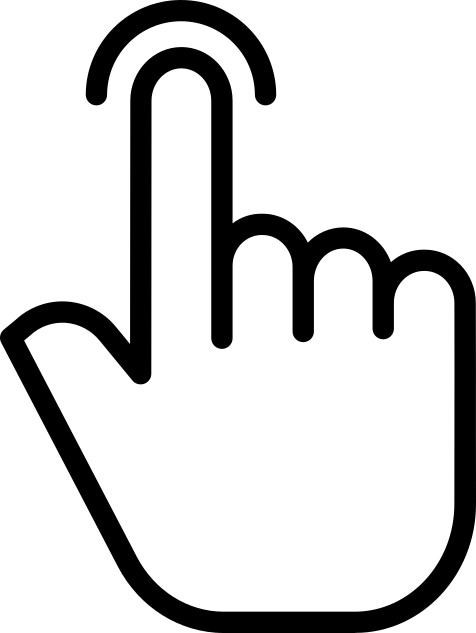
\includegraphics[width=0.03\textwidth]{static/dedo.png}} ;
         \node[factor, minimum size=1cm, xshift=3cm] (p3) {} ;
         
         \node[const, above=of p1, yshift=.15cm] (fp1) {$1/3$};
         \node[const, above=of p2, yshift=.15cm] (fp2) {$0$};
         \node[const, above=of p3, yshift=.15cm] (fp3) {$2/3$};
         \node[const, below=of p2, yshift=-.10cm, xshift=0.3cm] (dedo) {};        } 
\caption{Escribir}
\label{fig:monty_hall_condicional}
\end{figure}

Escribir ...



 
\section{Base empírica y selección de modelos}


% Parrafo

\subsection{Los datos como síntesis de las evidencias empíricas y formales.}
%
\begin{align*} \normalsize
\text{Habilidad} \underbrace{|}_{\hfrac{\text{Hipótesis}}{\text{indicadora}}} \underbrace{\text{Resultado}}_{\hfrac{\text{Evdencia}}{\text{empírica}}}, \underbrace{\text{Modelo causal}}_{\hfrac{\text{Evidencia}}{\text{teórica}}}
\end{align*}



\subsection{Teorema de Bayes}

El teorema de Bayes no lo escribió Bayes y tampoco es un teorema.
Es un corolario de la reglas de la probabilidad.
Las reglas de la probabilidad fueron expuestas por primera vez por Laplace a finales del 1700 y principios del 1800.
Por lo que sería más justo decir que es un corolario de Laplace.

\vspace{0.3cm}

\todo[inline, color=gray!50]{Hacer la demostración paso a paso}

.

.

.

.

\begin{equation*}
\underbrace{P(\text{Hip\'otesis }|\text{ Datos})}_{\text{\scriptsize Posteriori}} = \frac{\overbrace{P(\text{Datos }|\text{ Hip\'otesis})}^{\text{\scriptsize Verosimilitud}} \overbrace{P(\text{Hip\'otesis})}^{\text{\scriptsize Priori}} }{\underbrace{P(\text{Datos})}_{\text{\scriptsize Evidencia}}}
\end{equation*}




\subsection{La sorpresa como filtro de las creencias previas}

El teorema de Bayes no es necesario teóricamente, aunque en términos prácticos sea útil calcular la conjunta por partes (se entiende?).
Pero más allá de eso, expresar la condicional como teorema de Bayes permite interpretar mejor es que actualizamos las creencias.
Vemos la verosimilitud de Monty Hall.
Usando las reglas de la probabilidad podemos calcularla.

\subsection{Verosimilitud}

\begin{equation}
 P(s_2|r_i) = \frac{P(s_2|r_i)}{P(r_i)}
\end{equation}

\textbf{Notar que ahora la variable libre está del lado derecho del condicional.}

\todo[inline, color=gray!50]{Hacer pasos a paso el calculo de la verosimilitud.}

.

.

.

.


\begin{table}[H]
 \centering
$P(s_2|r_i)$ \\ \vspace{0.1cm} 
  \begin{tabular}{c|c|c|c} \setlength\tabcolsep{0.4cm} 
          & \, $r_1$ \, &  \, $r_2$ \, & \, $r_3$ \, \\ \hline 
   $s_2$ & $1/2$ & $0$ & $1$  \\ \hline
\end{tabular}
\caption{Escribir .. }
\label{tab:monty_hall_verosimilitud}
\end{table}

Escribir ...

\begin{framed}
\begin{align*}
  P(s_2|r_i, M) = \frac{\text{\textbf{Caminos que generan} $\bm{s_2}$ dada la hipótesis $r_i$ y el modelo}}{\text{\textbf{Caminos totales} dada la hipótesis $r_i$ y el modelo }}
 \end{align*}
 \end{framed}

  La verosimilitud es una predicción a priori suponiendo verdadera la hipótesis.
  Es predicción es justamente proporcional a la cantidad de caminos que ggeneran los datos dada la hipótesis.

 \subsection{Posterior}
 
 Escribir ... 
 
 \begin{align*}
   P(r_i|s_2) \propto P(r_i) P(s_2|r_i) 
  \end{align*}
 

 \begin{table}[H]
   \centering
  \begin{tabular}{c|c|c|c} \setlength\tabcolsep{0.4cm} 
        \phantom{$P(r_i|s_2) \propto$}  & \, $r_1$ \, &  \, $r_2$ \, & \, $r_3$ \, \\ \hline 
   $P(s_2|r_i)$ & $1/2$ & $0$ & $1$  \\ \hline
   $P(r_i)$ & $1/3$ & $1/3$ & $1/3$  \\ \hline
   $P(r_i|s_2) \propto$ & $1/6$ & $0$ & $1/3$  \\ \hline \hline
   $P(r_i|s_2) =$ & $1/3$ & $0$ & $2/3$  \\ \hline 
\end{tabular}
\caption{Escribir}
\label{tab:posterior}
\end{table}

\todo[inline, color=gray!50]{Explicar que es la sorpresa (1-verosimilitud) y hacer notar que el prior no que llega a ser posterior es proporcional a la sorpresa}

 \begin{framed}\centering
 $P(r_i|s_2) = $ Creencia inicial no filtrada por la sorpresa
 \end{framed}

  
\todo[inline, color=gray!50]{Hacer notar que la sorpresa es la fuente de información, lo que nos permite actulizar creencias.}
 

\subsection{Selección de las especies}

Evidencia

 Escribir
 
 \begin{equation*}
  P(s_2) = \sum_i P(s_2|r_i) P(r_i) = \frac{1}{2} \frac{1}{3} + 0 \frac{1}{3} + \frac{1}{1} \frac{1}{3} = 1/2 
 \end{equation*}
 
 Escribir
 
 \begin{framed} \centering
 Predicción a priori (hecha con todas las hipótesis)
 \end{framed}

 \todo[inline, color=gray!50]{Comparar con la verosimilitud. La evidencia también es una predicción a priori, pero hecha con todas las hipótesis. Mucho que explicar acá.}





\section{Conclusiones}

\begin{itemize}
\setlength\itemsep{-0.1cm}
%  \item \textbf{Evidencia formal:} organización de la materia.
%  \item \textbf{Evidencia empírica:} El comportamiento del mundo
 \item \textbf{Adaptación:} el cambio de la organización de la materia auto reproductiva debida al proceso de selección natural.
 \item \textbf{Conocimento:} la información contenida en la vida que sobrevive en el proceso evolutivo.
 \item \textbf{Datos:} Los datos como síntesis de las evidencias empíricas y formales. Siempre están cargados de teoría.
 \item \textbf{T-teoricidad:} T-teoricidad de los datos: T-teórico si todo procedimiento de determinación presupone la teorı́a T, y es T-no teórico si existe alguno que no la presupoga.
 \item \textbf{Base empírica:} La base empı́rica puede ampliarse o  reducirse aumentando o disminuyendo el conjunto de supuestos que una comunidad esta dispuesta a no poner en duda.
 \item \textbf{Intersubjetividad:} Sólo hay intersubjetividad, no objetividad. La ``objetividad'' aparece como resultado de una actividad constructiva entre sujetos y no como imposición del objeto al sujeto.
 \item \textbf{Honestidad:} La honestidad (máxima entropía dadas restricciones) como fuente de validez del conocimiento empírico.
 \item \textbf{Probabilidad:} La aplicación estricta de la teoría de la probabilidad como la generalización del principio de honestidad.
 \item \textbf{Teorema de Bayes:} El teorema de Bayes como generalización de la hipótesis indicadora, el puente de validez universal para determinar las evidencias empíricas y formales.
 \item \textbf{Likelihood:} El likelihood como generalización de la selección de la creencias previas.
 \item \textbf{Posterior:} El posterior como las creencias adaptadas (que sobrevivieron) al proceso de selección.
 \item \textbf{Evidencia:} La evidencia como cuantificación de la superviviencia total, generalización de la fuente e validez del conocimiento empírico.
\end{itemize}



\newpage

{\footnotesize

%\bibliographystyle{../../bibligrafia/plos2015.bst}
\bibliography{../../bibligrafia/Gaming/gaming.bib}

}

\chapter{Anexo}

\section{Teoría de la probabilidad}

\subsection{Sobre la diversa cantidad de sistemas axiomáticos del que se desprende la teoría de la probabilidad.}

Lo que Halpern rechaza de los teoremas tipo Cox no son su correctitud, sino la presunta ``naturalidad'' del sistema axiomático requerido para derivar las reglas de la probabilidad.
El axioma de densidad propuesto por Paris~\cite{paris1994} entre otros, i.e. de que las creencias sobre $H$ dado $E$ sea capaz de cubrir todas las graduaciones en $[0,1]$ para infinitas $E \in \mathbb{E}$, según Halpern~\cite{halpern1999-coxTheoremRevisited} no apelaría al ``sentido común'' por cuestiones relativas a la ontología del mundo.%, pero que si no se incoprora introduce un contra ejemplo al teorema de Cox~\cite{halpern1999-counterExampleCoxTheorem}.
La discusión por lo tanto no está señalando ningún problema del sistema matermático formal de los teorema tipo Cox, sino que propone un debate de caracter filosófico-epistemológico respecto de la elección de los axiomás y se relación aparente con el mundo natural.
En la segunda edición de su libro ``Reasoning about uncertainty'' Halpern presenta otro conjunto de axiomas basado.
Y concluye diciendo que si bien cada persona puede percibir diferente cuan convincente son el conjunto de axiomas propuestos, quizás el argumento más fuerte que demuestra la validez de la teoría de la probabilidad es que los filósofos han lllegado de varias forma independiente a la misma conclusión~\cite{halpern2017-RAU2}.
% %
% \begin{quotation}
% Different readers will probably have different feelings as to how compelling these and other defenses of probability really are.
% However, the fact that philosophers have come up with a number of independent justifications for probability is certainly a strong point in its favor. Much more effort has gone into justifying probability than any other approach for representing uncertainty. Time will tell if equally compelling justifications can be given for other approaches. In any case, there is no question that probability is currently the most widely accepted and widely used approach to representing uncertainty (Halpern~\cite{halpern2017-RAU2}).
% \end{quotation}








Según Halpern existen sistemas naturales que por su ontología no pueden generar infinitas evidencias $E$ distintas.




, que con junto con el el axioma que supone continuidad inducen la propiedad de asociatividad, o no se agrega un axioma que directamente suponga imponga asociatividad como hace \cite{cox1946}, entonces existe un contra-ejemplo al teorema~\cite{halpern1999-counterExampleCoxTheorem}.
Halpern rechaza la 

derivar el teorema de Cox.




Las criticas que hace Halpern al teorema de Cox tienen que ver con el sistemas axiomáti


has claimed to have constructed a counterexample to Cox's Theorem. Snow (The Reasonableness of Possibility from the Perspective of Cox, 2001) disagrees, saying that Cox implicitly made an assumption that negates the counterexample. Paris (The Uncertain Reasoner's Companion, 1994) seems to formalise this assumption, but the consequence is that the Cox-Jaynes probability function cannot have a finite domain.


Como luego aclara el mismo Halpern a raiz de las críticas que recibió su artículo~\cite{halpern1999-coxTheoremRevisited}, las demostraciones existentes del teorema de Cox,  ciertamente incluyen este requisito 

en los casos en los que no 
disallow a notion of belief that has
only finitely many gradations.






\


\end{document}
